\documentclass[a4paper, 12pt]{scrbook}

\usepackage{math-book}

\begin{document}

\frontmatter

\mainChapter{Lineáris algebra}\label{chap-01}

\bgroup
\color{gray!50!black}
\sffamily

A Matematika G2 kurzus első felében lineáris algebrával fogunk foglalkozni.
Ez a matematika azon területe, amely számos tudományágban és gyakorlati
alkalmazásban meghatározó szerepet játszik. Célunk a vektorterekkel, mátrixokkal
és lineáris leképezésekkel kapcsolatos alapvető ismeretek átadása, valamint a
lineáris egyenletrendszerek megoldhatóságának és megoldásának vizsgálata.
A vektorterek és a mátrixok a matematika és a mérnöki tudományok számos
területén alapvető szerepet töltenek be, segítenek leírni, megérteni
bonyolultabb rendszereket és struktúrákat. A lineáris egyenletrendszerek
megoldása szoros kapcsolatban áll a vektorterek és a mátrixok tulajdonságaival.
A mátrixok lehetővé teszik a lineáris transzformációk hatékony leírását.

A jegyzet ezen része a lineáris algebra alapjait igyekszik bemutatni: néhány
korábban tanult definíció felelevenítését követően, a vektorterek definíciója és
azok tulajdonságai, a mátrixműveletek elmélete, majd a lineáris
egyenletrendszerek különböző megoldási módszerei következnek, végül a lineáris
leképezések áttekintésével zárul. A célunk, hogy a témák megértéséhez szükséges
elméleti ismeretek mellett gyakorlati példákon keresztül is bemutassuk a
lineáris algebra széleskörű alkalmazási lehetőségeit.

Ez a jegyzet segít abban, hogy az Olvasó képet kapjon a lineáris algebra
fontosságáról és alkalmazásairól.

\chaptertoc
\egroup

\clearpage
\input{00-frontmatter/01-notations}

\mainmatter

\mainChapter{Lineáris algebra}\label{chap-01}

\bgroup
\color{gray!50!black}
\sffamily

A Matematika G2 kurzus első felében lineáris algebrával fogunk foglalkozni.
Ez a matematika azon területe, amely számos tudományágban és gyakorlati
alkalmazásban meghatározó szerepet játszik. Célunk a vektorterekkel, mátrixokkal
és lineáris leképezésekkel kapcsolatos alapvető ismeretek átadása, valamint a
lineáris egyenletrendszerek megoldhatóságának és megoldásának vizsgálata.
A vektorterek és a mátrixok a matematika és a mérnöki tudományok számos
területén alapvető szerepet töltenek be, segítenek leírni, megérteni
bonyolultabb rendszereket és struktúrákat. A lineáris egyenletrendszerek
megoldása szoros kapcsolatban áll a vektorterek és a mátrixok tulajdonságaival.
A mátrixok lehetővé teszik a lineáris transzformációk hatékony leírását.

A jegyzet ezen része a lineáris algebra alapjait igyekszik bemutatni: néhány
korábban tanult definíció felelevenítését követően, a vektorterek definíciója és
azok tulajdonságai, a mátrixműveletek elmélete, majd a lineáris
egyenletrendszerek különböző megoldási módszerei következnek, végül a lineáris
leképezések áttekintésével zárul. A célunk, hogy a témák megértéséhez szükséges
elméleti ismeretek mellett gyakorlati példákon keresztül is bemutassuk a
lineáris algebra széleskörű alkalmazási lehetőségeit.

Ez a jegyzet segít abban, hogy az Olvasó képet kapjon a lineáris algebra
fontosságáról és alkalmazásairól.

\chaptertoc
\egroup

\clearpage
\clearpage
\section{Alapfogalmak}\label{sec-03-01}

\begin{definition}[Gömbkörnyezet]
  Legyen $\rvec p \in \Reals^n$. Ekkor a $\rvec p$ pont $\varepsilon$ sugarú
  nyílt környezetén (gömbkörnyezetén) a
  $$
    B_\varepsilon(\rvec p) := \{
    \rvec x \in \Reals^n \mid | \rvec x - \rvec p | < \varepsilon
    \}
    \text{ halmazt értjük.}
  $$
\end{definition}

\begin{note}
  A tobábbiakban $\mathbb E^n$ jelölje az $n$ dimenziós euklideszi teret.
\end{note}

\begin{definition}[Pontsorozat konvergenciája]
  A $(\rvec p_n)$ $\mathbb E^n$-beli pontsorozat konvergens, ha
  $\exists \rvec p \in \mathbb E^n$, hogy $\forall \varepsilon > 0$ esetén
  $\exists N(\varepsilon)$ küszöbindex, hogy $n > N(\varepsilon)$ esetén
  $\rvec p_n \in B_\varepsilon(\rvec p)$.

  Ekkor a $\rvec p$ pontot a sorozat határértékének, vagy határpontjának
  nevezzük.
\end{definition}

\begin{theorem}[Bolzano-Weierstrass-féle kiválasztási tétel]
  Végtelen, korlátos, $\Reals^n$-beli ponthalmazból kiválasztható konvergens
  pontsorozat részsorozata. Ezen sorozat határértéke (határpontja) a ponthalmaz
  torlódási pontja.

  \begin{proof}
    \vspace{8em}
  \end{proof}
\end{theorem}

\begin{blueBox}
  \sftitle{Többváltozós függvények jelölése:}

  Legyen $\rvec f: \Reals^n \to \Reals^k$ függvény. Ekkor a függvény az alábbi
  formában írható fel:
  $$
    \begin{bmatrix}
      x_1 \\ x_2 \\ \vdots \\ x_n
    \end{bmatrix} \mapsto \rvec f(x_1; x_2; \ldots; x_n) = \begin{bmatrix}
      f_1 (x_1; x_2; \ldots; x_n) \\
      f_2 (x_1; x_2; \ldots; x_n) \\
      \vdots                      \\
      f_k (x_1; x_2; \ldots; x_n)
    \end{bmatrix}
    \text,
  $$
  ahol az $f_i: \Reals^n \to \Reals, i \in \{1;2;\dots;k\}$ függvényeket
  komponensfüggvényeknek nevezzük.

  \sftitle{Speciális elnevezések:}

  \def\arraystretch{1.33}
  \begin{tabular}{ll}
    \bullet \; $\rvec f: \Reals^n \to \Reals^k$             & vektor-vektor függvény,
    \\
    \bullet \; $\rvec f: \Reals^n \to \Reals^{\phantom{k}}$ & vektor-skalár függvény,
    \\
    \bullet \; $\rvec f: \Reals^{\phantom{n}} \to \Reals^k$ & skalár-vektor függvény.
  \end{tabular}
\end{blueBox}

\begin{definition}[Többváltozós függvény határértéke]
  Tekintsük az $\rvec f: \Reals^n \to \Reals^k$ leképezést. Azt mondjuk, hogy az
  $f$ határértéke $\rvec a \in \Reals^n$ pontban $\rvec A \in \Reals^k$, ha az
  $\rvec A$ tetszőleg $\varepsilon > 0$ sugarú gömbkörnyezetéhez létezik az
  $\rvec a$-nak olyan $\delta(\varepsilon)$ sugarú gömbkörnyezete, hogy
  $$
    \rvec x \in B_{\delta(\varepsilon)}(\rvec a) \setminus \{\rvec a\}
    \quad \Rightarrow \quad
    \rvec f(\rvec x) \in B_\varepsilon(\rvec A)
    \text.
  $$
\end{definition}

\begin{definition}[Többváltozós függvény folytonossága]
  Azt mondjuk, hogy az $\rvec f: \Domain_f \subset \Reals^n \to \Reals^k$ leképezés
  folytonos az értelmezési tartományának egy belső pontjában
  ($\rvec a \in \Domain_f$), ha az adott pontbeli határértéke megegyezik
  az adott pontbeli függvényértékkel, vagyis
  $$
    \lim_{\rvec x \to \rvec a} \rvec f(\rvec x) = \rvec f(\rvec a)
    \text.
  $$
\end{definition}

\begin{theorem}[Átviteli elv egyváltozós függvényekre]
  Az $f$ függvény határértéke az $a \in \Domain_f$ pontban akkor és csak akkor
  $A$, ha $\forall x_n \to a$ sorozat esetén $f(x_n) \to A$.
\end{theorem}

\begin{theorem}[Az átviteli elv általánosítása]
  Az $\rvec f: \Reals^n \to \Reals^k$ függvény határértéke az $\rvec a \in \Reals^n$
  pontban akkor és csak akkor $\rvec A \in \Reals^k$, ha
  $\forall \rvec x_n \to \rvec a$ sorozat esetén
  $\rvec f(\rvec x_n) \to \rvec A$.
\end{theorem}

\begin{definition}[Többváltozós függvény differenciálhatósága]
  Legyen $I \in \Reals^n$ nyílt halmaz, $\rvec f: I \to \Reals^k$ leképezés.
  Azt mondjuk, hogy az $\rvec f$ differenciálható az $\rvec a \in I$ pontban, ha
  $\exists \rvec \mathscr A: \Reals^n \to \Reals^k$ lineáris leképezés és
  $\rvec w: \Reals^n \to \Reals^k$ függvény, hogy
  $$
    \rvec w(\nvec) = \nvec
    \quad\text{és}\quad
    \lim_{\rvec \|h\| \to 0} \frac{
      \|\rvec w(\rvec h)\|
    }{
      \|\rvec h\|
    }
    \text,\quad \text{hogy} \quad
    \rvec f(\rvec x) - \rvec f(\rvec A)
    = \rvec \mathscr A(\rvec x - \rvec a) + \rvec w(\rvec x - \rvec a)
    \text.
  $$
\end{definition}

\begin{statement}
  Ha az $\rvec f: I \subset \Reals^n \to \Reals^k$ függvény differenciálható az
  $\rvec a \in I$ pontban, akkor ott folytonos is.

  \begin{proof}
    Legyen $\rvec h = \rvec x - \rvec a$, ekkor
    $\displaystyle
      \rvec f(\rvec x) - \rvec f(\rvec a)
      = \rvec \mathscr A(\rvec h) + \rvec w(\rvec h)
      = \rvec \mathscr A(\rvec h) + \frac{\rvec w(\rvec h) \|\rvec h\|}{\|\rvec h\|}
      \text.
    $
    \\[2mm]
    Ha $\rvec h \to \nvec$, akkor $\rvec w(\rvec h) / \|\rvec h\| \to \nvec$,
    azaz $\|\rvec f(\rvec a + \rvec h) - \rvec f(\rvec a)\|$ tetszőlegesen
    kicsivé tehető, hiszen $\mathscr A(\nvec) = \nvec$ tetszőleges lineáris
    leképezésre igaz. Az állítás így igaz.
  \end{proof}
\end{statement}

\begin{statement}
  Ha létezik az $\rvec f: I \subset \Reals^n \to \Reals^k$ függvénynek az
  $\rvec a \in I$ pontbeli deriváltja, akkor az $\mathscr A$ lineáris lekézezés
  egyértelmű.

  \begin{proof}[Indirekt módon]
    Tegyük fel, hogy $\rvec \mathscr A_1: \Reals^n \to \Reals^k$ és
    $\rvec \mathscr A_2: \Reals^n \to \Reals^k$ két különböző lineáris leképezés
    egyaránt az $\rvec f$ függvénynek az $\rvec a$ pontbeli deriváltja. Ekkor
    $$
      \lim_{\|\rvec h\| \to 0} \frac{
        \|\rvec f(\rvec a + \rvec h) - \rvec f(\rvec a) - \rvec \mathscr A_1(\rvec h)\|
      }{
        \|\rvec h\|
      }
      \quad\text{ és }\quad
      \lim_{\|\rvec h\| \to 0} \frac{
        \|\rvec f(\rvec a + \rvec h) - \rvec f(\rvec a) - \rvec \mathscr A_2(\rvec h)\|
      }{
        \|\rvec h\|
      }
      \text.
    $$
    Vonjuk ki egymásból a két kifejezést:
    $$
      \lim_{\|\rvec h\| \to 0} \frac{
        \|\rvec \mathscr A_1(\rvec h) - \rvec \mathscr A_2(\rvec h)\|
      }{
        \|\rvec h\|
      }
      = 0
      \text.
    $$
    Mivel $\rvec \mathscr A_1$ és $\rvec \mathscr A_2$ lineáris leképezések,
    ezért a különbségük is az, ebből
    $$
      \rvec \mathscr A_1(\rvec h) - \rvec \mathscr A_2(\rvec h)
      = \underbrace{(\rvec \mathscr A_1 - \rvec \mathscr A_2)}_{\mathscr B}(\rvec h)
      \text.
    $$
    Vizsgáljuk a $\rvec h = \lambda \rvec u$ esetet. Ekkor, ha
    $\rvec h \to \nvec$, akkor $\lambda \to 0$ is igaz. Tehát
    $$
      \lim_{\lambda \to 0} \frac{\mathscr B(\lambda \rvec u)}{\|\lambda \rvec u\|}
      = \lim_{\lambda \to 0} \frac{\lambda \mathscr B(\rvec u)}{|\lambda| \, \|\rvec u\|}
      = \nvec
      \text.
    $$
    Mivel tetszőleges $\rvec u \in \Reals^n$ esetén a
    $\lambda / |\lambda| = \pm 1$, ezért $\mathscr B(\rvec u) = \nvec$.
    Azaz $\mathscr B$ lineáris leképezés, méghozzá a nulla leképezés, ezért
    $\rvec \mathscr A_1 = \rvec \mathscr A_2$, ami ellentmond a feltételezésnek.
  \end{proof}
\end{statement}

\begin{definition}[Többváltozós függvény differenciálhatósága]
  Az $\rvec f: \Reals^n \to \Reals^k$ leképezés differenciálható az értelmezési
  tartományának egy adott pontjában, ha ebben a pontban a komponensfüggvényei
  is differenciálhatóak.
\end{definition}

\begin{statement}
  Legyen $\rvec f: \Reals^n \to \Reals^k$ és $\rvec g: \Reals^k \to \Reals^m$
  differenciálhatóak az $\rvec a \in \Domain_f \cap \Domain_g$ pontban. Ekkor
  az $\rvec f + \rvec g$ is differenciálható az $\rvec a$ pontban, és
  $$
    (\rvec f + \rvec g)'(\rvec a) = \rvec f'(\rvec a) + \rvec g'(\rvec a)
    \text.
  $$
\end{statement}

\begin{statement}
  Legyen $\rvec f: \Reals^n \to \Reals^k$ differenciálható az
  $\rvec a \in \Domain_f$ pontban, és $\lambda \in \Reals$. Ekkor a
  $\lambda \rvec f$ is differenciálható az $\rvec a$ pontban, és
  $$
    (\lambda \rvec f)'(\rvec a) = \lambda \rvec f'(\rvec a)
    \text.
  $$
\end{statement}

% Chain rule
\begin{statement}
  Legyen $\rvec f: \Reals^n \to \Reals^k$ és $\rvec g: \Reals^k \to \Reals^m$
  leképezések, $\forall x \in \Domain_f$-re $f(x) \in \Domain_g$, továbbá
  $\rvec f$ differenciálható az $\rvec a \in \Domain_f$ pontban és
  $\rvec g$ differenciálható az $\rvec f(\rvec a)$ pontban. Ekkor a
  $\rvec g \circ \rvec f$ is differenciálható az $\rvec a$ pontban, és
  $$
    (\rvec g \circ \rvec f)'(\rvec a) = \rvec g'(\rvec f(\rvec a)) \circ \rvec f'(\rvec a)
    \text.
  $$
\end{statement}
\section{Relációk, leképezések, függvények}

\begin{definition}[Descartes-szorzat]
  Az $A$ és $B$ halmazok Descartes-szorzatán az $A$ és $B$ halmaz elemeiből álló
  \textbf{összes rendezett elempár}ok halmazát értjük:
  \[
    A \times B := \Big\{\;
    (a; b) \;\Big|\; (a \in A) \land (b \in B)
    \;\Big\}
    \text.
  \]
\end{definition}

\begin{example}
  Legyen $A = \{1;2\}$ és $B = \{a;b\}$, ekkor az $A \times B$
  Descartes-szorzat:
  \[
    A \times B = \Big\{\;
    (1; a); (1; b); (2; a); (2; b)
    \;\Big\}
    \text.
  \]

\end{example}

\begin{definition}[Binér reláció]
  Az $A \times B$ szorzathalmaz $T \subset A \times B$ részhalmazát az $A$ és
  $B$ közötti binér (kételemű) relációnak hívjuk. Ha $(a; b) \in T$, akkor azt
  mondjuk, hogy $a$ és $b$ relációban vannak, és ezt $aTb$-vel jelöljük.
\end{definition}

\begin{definition}[Reláció értelmezési tartománya, értékkészlete és inverze]
  Legyen $ T\subset A\times B$ egy reláció, ekkor
  \begin{center}
    \def\arraystretch{1.5}
    \addtolength{\tabcolsep}{-0.25em}
    \begin{tabular}{
        >{$}r<{: = \Big\{$}
        >{$}c<{$}
        >{$\Big|$}c
        >{$}c<{$}
        >{$\Big\}$}c
        >{--}c
        l
      }
      \Domain_T
       & a \in A
       &         & \exists b \in B: (a;b) \in T
       &         &                              & a reláció értelmességi tartománya,
      \\
      \Range_T
       & b \in B
       &         & \exists a \in A: (a;b) \in T
       &         &                              & a reláció értékkészlete,
      \\
      T^{-1}
       & (b;a)
       &         & (a;b) \in T
       &         &                              & a reláció inverze.
    \end{tabular}

  \end{center}
\end{definition}

\begin{definition}[Ekvivalenciareláció]
  Legyen $A \neq \emptyset$, a $T \subset A \times A$ relációt ekvivalencia%
  relációnak mondjuk, ha teljesülnek az alábbiak:
  \begin{itemize}
    \item \textbf{reflexivitás} -- $\forall A \in A$ esetén $(a; a) \in T$,
    \item \textbf{szimmetria} -- ha $(a; b) \in T$, akkor $(b; a) \in T$,
    \item \textbf{tranzitivitás} -- ha $(a; b) \in T$ és $(b; c) \in T$, akkor
          $(a; c) \in T$.
  \end{itemize}
\end{definition}

\begin{theorem}[Ekvivalencia osztályok]
  Minden $A \times A$ halmazon adott ekvivalenciareláció diszjunkt halmazokra
  bontja fel az A halmazt, ezeket a diszjunkt halmazokat ekvivalencia%
  osztályoknak nevezzük.
\end{theorem}

\begin{example}
  \samepage
  Két természetes szám relációban van egymással, ha hárommal osztva azonos
  maradékot adnak.
  \begin{center}
    \begin{tikzpicture}[ultra thick]
      \node[
        circle,
        minimum size=3.5cm,
        draw=primaryColor,
        fill=primaryColor!10
      ] (C) at (0,0) {};

      \coordinate (1) at (80:1.75);
      \coordinate (2) at (100:1.75);

      \draw[primaryColor, fill=primaryColor!10]
      ($(2)+(1mm,6mm)$)
      arc (90:180:1mm)
      -- (2)
      arc (100:80:1.75)
      -- ++(0,5mm)
      arc (0:90:1mm)
      -- cycle
      ;

      \node at (0,2.025) {$\mathbb N$};


      \draw[secondaryColor] (170:1.75) .. controls (40:.35) .. (290:1.75)
      coordinate[pos=0.6] (A);

      \draw[secondaryColor] (A) .. controls (30:.75) .. (90:1.75);

      \foreach \angle/\label in {110/0, 230/1, 345/2}{
          \node at (\angle:1) {$\overline\label$};
        }
    \end{tikzpicture}
  \end{center}
\end{example}

\begin{definition}[Függvény]
  A $T \subset A \times B$ binér relációt leképezésnek/függvénynek mondjuk, ha
  \[
    (a; b) \in T \land (a; c)\in T \Rightarrow b = c
    \text.
  \]
  Jelölés: $f: A \rightarrow B$, ahol $A$ az értelmezési tartomány ($\Domain_f$)
  és $B$ az értékkészlet ($\Range_f$).
\end{definition}

\begin{definition}[Bijekció]
  Az $f : A \rightarrow B$ kölcsönösen egyértelmű (egy-egyértelmű, bijektív), ha
  \begin{itemize}
    \item \textbf{injektív}, vagyis $f(a_1) = f(a_2) \Rightarrow a_1 = a_2$,
          valamint
    \item \textbf{szürjektív}, vagyis $\forall b \in B$ esetén $\exists a \in A:
            f(a) = b$.
  \end{itemize}
\end{definition}

\begin{note}
  Ha az $f: A \rightarrow B$ bijektív, akkor az $f^{-1}: B \rightarrow A$
  leképezést $f$ \textbf{inverz leképezés}ének hívjuk.
\end{note}

\begin{example}
  Az $f: \Reals \rightarrow (0; +\infty), x \mapsto e^x$ függvény bijektív,
  inverze a természetes alapú logaritmus: $f^{-1}: (0; +\infty) \rightarrow
    \Reals, x \mapsto \ln x$.

  \begin{center}
    \begin{tikzpicture}[ultra thick]
      % COORDINATE SYSTEM
      \draw[-to, draw=primaryColor] (-2.5,0) -- (3,0) node[above left] {$x$};
      \draw[-to, draw=primaryColor] (0,-2.5) -- (0,3) node[below left] {$y$};

      \draw[very thick, gray, dashed] (-2,-2) -- (2,2);

      % PLOT EXP(X)
      \draw plot[domain=-2.25:0.85, samples=25, smooth, draw=secondaryColor]
      (\x, {exp(\x)})
      node[above right] {$e^x$}
      ;
      % PLOT LN(X)
      \draw plot[domain=0.10:2.5, samples=25, smooth, draw=secondaryColor]
      (\x, {ln(\x)})
      node[above right] {$\ln x$}
      ;
    \end{tikzpicture}
  \end{center}
\end{example}

% \clearpage
\clearpage
\section{A számfogalom kiépítése}\label{sec-01-03}

\begin{blueBox}
  \bgroup
  \sffamily\bfseries Peano-axiómák:
  \egroup

  Legyen $ \mathbb N \neq \emptyset$, $\mathbb N$-t a természetes számok
  halmazának, elemeit természetes számoknak mondjuk, ha teljesülnek az alábbiak:
  \begin{enumerate}
    \item legyen adva egy $\varphi : \mathbb N \rightarrow \mathbb N$ leképezés,
    \item $\varphi$ injektív : $\varphi(a) = \varphi(b) \Rightarrow a = b$,
    \item $\exists$ $\mathbb N$-nek egy kitüntetett eleme, ez a $0$,
    \item a $0$-nak nincs ősképe, azaz $\nexists n \in \mathbb N : \varphi(n) =
            0$,
    \item a teljes indukció elve teljesül, azaz ha $H \subseteq \mathbb N$ és
          \begin{enumerate}
            \item $0 \in H$,
            \item $n \in H \Rightarrow \varphi(n) \in H$,
          \end{enumerate}
          akkor $H = \mathbb N$.
  \end{enumerate}
\end{blueBox}

\begin{blueBox}
  A természetes számok halmazát ekvivalenciarelációkkal ellátva megkapjuk a
  középiskolában megismert számhalmazokat:
  \begin{itemize}
    \item $\mathbb Z$ : az egész számok halmaza
          ($\mathbb N \times \mathbb N$),
    \item $\mathbb Q$ : a racionális számok halmaza
          ($\mathbb Z \times \mathbb Z$),
    \item $\mathbb Q^*$ : az irracionális számok halmaza,
    \item $\Reals$ : a valós számok halmaza
          ($\mathbb Q \cup \mathbb Q^*$).
  \end{itemize}

  \begin{center}
    \begin{tikzpicture}[ultra thick, draw=primaryColor]
      % SETS WITH LABELS
      \draw         (0.00,0) ellipse (1.5 and 1)    node[right=0.75cm] {$\mathbb N$};
      \draw         (0.75,0) ellipse (2.5 and 1.67) node[right=1.75cm] {$\mathbb Z$};
      \draw         (1.50,0) ellipse (3.5 and 2.33) node[right=2.75cm] {$\mathbb Q$};
      \draw[dashed] (2.25,0) ellipse (4.5 and 3)    node[right=3.75cm] {}           ;
      \draw         (3.00,0) ellipse (5.5 and 3.67) node[right=4.75cm] {$\Reals   $};

      % HELPER LINES FOR IRRATIONALS AND TRANSCENDENTALS
      \draw[dashed, gray, very thick] (8.50,0) -- ++(0,-4.85);
      \draw[dashed, gray, very thick] (6.75,0) -- ++(0,-3.90);
      \draw[dashed, gray, very thick] (5.00,0) -- ++(0,-4.85);

      \begin{scope}[font=\scriptsize]
        % IRRATIONALS
        \draw[to-to, draw=secondaryColor, very thick]
        (5.00,-4.70) -- ++(3.50,0)
        node [midway, above] {irracionális};

        % TRANSCENDENTALS
        \draw[to-to, draw=secondaryColor, very thick]
        (6.75,-3.75) -- ++(1.75,0)
        node [midway, above] {transzcendens};
      \end{scope}

      % NATURAL EXAMPLES
      \node (N) at (-0.85,0) {$1$};
      \node[above right] at (N.100) {$0$};
      \node[below right] at (N.260) {$2$};

      % INTEGERS EXAMPLES
      \node (Z) at (2,+0.5) {$-1$};
      \node (Z) at (2,-0.5) {$-2$};

      % RATIONALS EXAMPLES
      \node (Q) at (3.75,+0.5) {$\sfrac{1}{2}$};
      \node (Q) at (3.75,-0.5) {$\sfrac{2}{3}$};

      % IRRATIONALS EXAMPLES
      \node (I) at (5.75,+0.5) {$\sqrt{2}$};
      \node (I) at (5.75,-0.5) {$\frac{1 + \sqrt5}{2}$};

      % TRANSCENDENTALS EXAMPLES
      \node (T) at (7.5,+0.5) {$\pi$};
      \node (T) at (7.5,-0.5) {$e$};
    \end{tikzpicture}
  \end{center}
\end{blueBox}

\begin{note}
  A \textbf{transzcendens} számok olyan irracionális, valós számok, amelyek
  nem algebraiak, azaz nem valamely racionális együtthatós polinom gyökei. Ilyen
  szám pélául a $\pi$.
\end{note}

\clearpage
\begin{blueBox}
  \sftitle{A valós számok axiómarendszere:}

  Értelmezzük két bináris műveletet, az összeadást ($+$) és a szorzást
  ($\cdot$), valamint egy relációt ($>$).

  \bgroup
  \def\arraystretch{2}
  \newcounter{tctr}
  \begin{tabular}{
      @{\stepcounter{tctr}\makebox[2.25em][r]{\arabic{tctr}.\;\;}}
      >{$}l<{$}
      >{\makebox[2.5em][c]{$\sim$}}l
    }
    a + b = b + a
     & $+$ kommutatív,
    \\
    (a + b) + c = a + (b + c)
     & $+$ asszociatív,
    \\
    \exists! 0 \in \Reals : a + 0 = a
     & $+$ egységelem,
    \\
    \forall a \in \Reals : \exists -a \in \Reals : a + (-a) = 0
     & $+$ inverz elem,
    \\
    a \cdot b = b \cdot a
     & $\cdot$ kommutatív,
    \\
    (a \cdot b) \cdot c = a \cdot (b \cdot c)
     & $\cdot$ asszociatív,
    \\
    \exists! 1 \in \Reals : a \cdot 1 = a
     & $\cdot$ egységelem,
    \\
    \forall a \in \Reals \setminus \{0\} : \exists a^{-1} \in \Reals :
    a \cdot a^{-1} = 1
     & $\cdot$ inverz elem,
    \\
    a \cdot (b + c) = a \cdot b + a \cdot c
     & disztributivitás,
    \\
    \forall a, b \in \Reals : a < b \vee a = b \vee b < a
     & trichotómia,
    \\
    \forall a, b, c \in \Reals : a < b \land b < c \Rightarrow a < c
     & $<$ tranzitivitás,
    \\
    \forall a, b, c \in \Reals : a < b \Rightarrow a + c < b + c
     & $+$ monotonitás,
    \\
    \forall a, b, c \in \Reals : a < b \land 0 < c \Rightarrow
    a \cdot c < b \cdot c
     & $\cdot$ monotonitás,
    \\
    \forall a \in \Reals : \exists n \in \mathbb N : a < n
     & Arkhimédész-féle rendezés,
    \\
    a_n \leq a_{n+1} \land b_n \geq b_{n+1}: \bigcap\limits_{n = 1}^{\infty}
    \left[ a_n; b_n \right] \neq \emptyset
     & Cantor-axióma,
  \end{tabular}
  \egroup
\end{blueBox}

\begin{blueBox}
  \begin{itemize}
    \item $2 - 4$: csoport,
    \item $1 - 4$: Abel-csoport,
    \item $1 - 9$: test,
    \item $1 - 13$: rendezett test,
    \item $1 - 14$: arkhimédészien rendezett test,
    \item $1 - 15$: teljes rendezett test.
  \end{itemize}
\end{blueBox}

\begin{statement}
  A $\mathbb Q$ és $\mathbb Q^*$ sűrű.
\end{statement}
\clearpage
\section{Halmazok számossága}\label{sec-01-04}

\begin{definition}[Azonos számosságú halmazok]
  Ha két halmaz, $A$ és $B$ között kölcsönösen egyértelmű megfeleltetés hozható
  létre, akkor azt mondjuk, hogy a két halmaz számossága azonos. Jelölése:
  $\card A = \card B$.
\end{definition}

\begin{note}
  A számosság ekvivalenciareláció.
\end{note}

\begin{definition}[Véges halmaz]
  Az $A$ halmaz véges, ha $\exists n \in \mathbb N$, hogy $\card A = \card \; \{
    1; 2; \dots; n \}$, vagy ha $A = \emptyset$.
\end{definition}

\begin{note}
  Ha nincs olyan $n$ természetes szám, amelyre az $A \neq \emptyset$ halmaz
  ekvivalens volna az $\{ 1; 2; \dots; n \}$ halmazzal, akkor az $A$ halmazt
  végtelen számosságúnak mondjuk. Létezik megszámlálhatóan és
  megszámlálhatatlanul végtelen halmaz.
  \vspace{-5mm}
  \begin{center}
    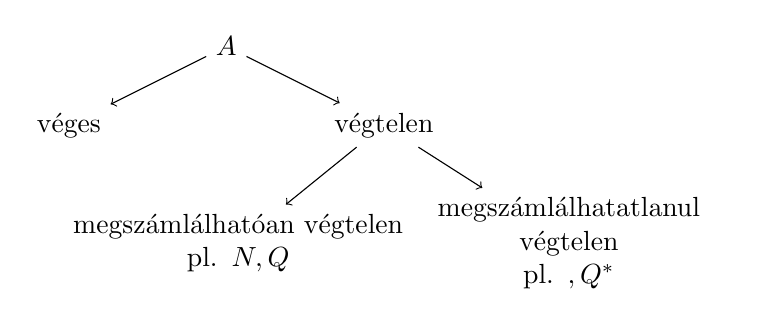
\begin{tikzpicture}
      % FIRST ROW
      \node (1) at (0,0) {$\card A$};

      % SECOND ROW
      \node (21) at (-2,-1) {véges};
      \node (22) at (2,-1) {végtelen};

      % CONNECT 1 -> 2
      \draw[->] (1) -- (21);
      \draw[->] (1) -- (22);

      % THIRD ROW
      \node[text width=4.5cm, align=center] (31) at (0.15,-2.5)
      {megszámlálhatóan végtelen\\pl. $\mathbb N, \mathbb Q$};
      \node[text width=4.5cm, align=center] (32) at (4.35,-2.5)
      {megszámlálhatatlanul végtelen\\pl. $\Reals, \mathbb Q^*$};

      % CONNECT 2 -> 3
      \draw[->] (22) -- (31);
      \draw[->] (22) -- (32);
    \end{tikzpicture}
  \end{center}
\end{note}

\begin{theorem}[Racionális számok halmazának számossága]
  A racionális számok halmaza megszámlálhatóan végtelen.

  \begin{proof}[Cantor átlós módszere]
    \begin{minipage}{.5\textwidth}
      Minden pozitív racionális szám felírható tört alakban, ahol a nevező és a
      számláló is egész szám, ráadásul ezek relatív prímek.
      \\[.33em]
      Ezeket a törteket rendezzük egy olyan táblázatba, ahol az $n$ sorban az
      $m$ oszlopban az $\sfrac{m}{n}$ tört áll. Ezeket a törteket az ábrán
      jelöl módszerrel sorba állítjuk, sorrendjük szerint pedig egyértelműen
      megfeleltethetők a természetes számoknak.
      \\[.33em]
      Könnyen belátható, hogy ez a módszer az összes racionális számra
      is kiterjeszthető, tehát a racionális számok halmaza valóban
      megszámlálhatóan végtelen.
      %\begin{noindent}
    \end{minipage}\hfill%
    \begin{minipage}{.425\textwidth}
      % \end{noindent}
      \begin{tikzpicture}[
          decoration={
              markings,
              mark=at position 0.5 with {\arrow{>}
                }
            }
        ]
        \draw[ultra thick, secondaryColor] (.5,-.5) rectangle (6.5,-7.5);

        \foreach \y in {1,...,6}{
            \foreach \x in {1,...,5}{
                \node (\x\y) at (\x,-\y) {$\sfrac{\x}{\y}$};
              }
          }

        \foreach \y in {1,...,6} {
            \node (6\y) at (6,-\y) {$\hdots$};
          }
        \foreach \x in {1,...,5}{
            \node (\x7) at (\x,-7) {$\vdots$};
          }
        \node(67) at (6,-7) {$\ddots$};

        \coordinate (P) at (11);
        \foreach \c in {12, 21, 31, 22, 13, 14, 23, 32, 41, 51, 42, 33, 24, 15, 16, 25, 34, 43, 52, 61}{
            \draw[postaction={decorate}, primaryColor, thick, opacity=0.5] (P) -- (\c.center);
            \coordinate (P) at (\c);
          }
      \end{tikzpicture}
    \end{minipage}
  \end{proof}
\end{theorem}

% \begin{theorem}[Valós számok halmazának számossága]
%   A valós számok halmaza nem megszámlálhatóan végtelen.
% \end{theorem}

% Ponthalmazok
\begin{blueBox}
  \sftitle{Fontosabb jelölések:}
  \begin{itemize}
    \item Nyílt halmaz jelölése: $(x; y) = ]x; y[$.
    \item Zárt halmaz jelölése: $[x; y]$.
    \item Az $a$ pont $\varepsilon$ sugarú környezete: $K(a; \varepsilon) := (a
          - \varepsilon; a + \varepsilon)$ \\ (ezzel ekvivalens: $|x-a| <
          \varepsilon$).
  \end{itemize}

  \begin{center}
    \begin{tikzpicture}
      % ARROW
      \draw[-to, ultra thick, secondaryColor] (-2,0) -- (2,0);

      % a point
      \draw[draw=primaryColor, ultra thick] (0,-1mm) -- ++(0,2mm)
      node[above] {$a$};

      % OPEN INTERVAL
      \draw[draw=primaryColor, ultra thick] (+10:1.25) arc (+10:-10:1.25)
      node[below] {$a + \varepsilon$};
      \draw[draw=primaryColor, ultra thick] (170:1.25) arc (170:190:1.25)
      node[below] {$a - \varepsilon$};
    \end{tikzpicture}
  \end{center}
\end{blueBox}

\begin{definition}[Alsó és felső korlát]
  A felülről korlátos $H$ halmaz legkisebb felső korlátja: supremum, jele: $\sup
    H$.
  \\
  Az alulról korlátos $H$ halmaz legnagyobb alsó korlátja: infimum, jele: $\inf
    H$.
\end{definition}

\begin{theorem}[Korlátos halmaz szuprémuma]
  Felülről korlátos nemüres halmaznak mindig van szuprémuma.
\end{theorem}

\begin{theorem}[Korlátos halmaz infimuma]
  Alulról korlátos nemüres halmaznak mindig van infimuma.
\end{theorem}
\vfill
\begin{questions}[section.1.5]
  \begin{enumerate}
    \item Mikor mondjuk, hogy egy halmaz jól definiált?

    \item Válassza ki az alábbi halmazok közül azokat, amelyek jól definiáltak!
          \begin{enumerate}
            \item A magas férfihallgatók,
            \item azon valós számok, amelyek négyzete nem kisebb háromnál,
            \item a viharos erejű szelek,
            \item a poliéderek.
          \end{enumerate}

    \item Definiálja a következő fogalmakat: üreshalmaz, halmaz komplementere,
          részhalmaz, halmazok metszete, uniója

    \item Definiálja két halmaz Descartes-szorzatát!

    \item Hány részhalmaza van egy $n$ elemű halmaznak?

    \item Zárt-e az irracionális számok halmaza az összeadásra nézve?

    \item Alulról korlátos-e a természetes számok halmaza? És felülről?

    \item Adjon példát véges halmazokra!

    \item Adjon példát megszámlálhatóan végtelen számosságú halmazokra!
  \end{enumerate}
\end{questions}

\mainChapter{Lineáris algebra}\label{chap-01}

\bgroup
\color{gray!50!black}
\sffamily

A Matematika G2 kurzus első felében lineáris algebrával fogunk foglalkozni.
Ez a matematika azon területe, amely számos tudományágban és gyakorlati
alkalmazásban meghatározó szerepet játszik. Célunk a vektorterekkel, mátrixokkal
és lineáris leképezésekkel kapcsolatos alapvető ismeretek átadása, valamint a
lineáris egyenletrendszerek megoldhatóságának és megoldásának vizsgálata.
A vektorterek és a mátrixok a matematika és a mérnöki tudományok számos
területén alapvető szerepet töltenek be, segítenek leírni, megérteni
bonyolultabb rendszereket és struktúrákat. A lineáris egyenletrendszerek
megoldása szoros kapcsolatban áll a vektorterek és a mátrixok tulajdonságaival.
A mátrixok lehetővé teszik a lineáris transzformációk hatékony leírását.

A jegyzet ezen része a lineáris algebra alapjait igyekszik bemutatni: néhány
korábban tanult definíció felelevenítését követően, a vektorterek definíciója és
azok tulajdonságai, a mátrixműveletek elmélete, majd a lineáris
egyenletrendszerek különböző megoldási módszerei következnek, végül a lineáris
leképezések áttekintésével zárul. A célunk, hogy a témák megértéséhez szükséges
elméleti ismeretek mellett gyakorlati példákon keresztül is bemutassuk a
lineáris algebra széleskörű alkalmazási lehetőségeit.

Ez a jegyzet segít abban, hogy az Olvasó képet kapjon a lineáris algebra
fontosságáról és alkalmazásairól.

\chaptertoc
\egroup

\clearpage
\section{Fogalmak, definíciók}

\begin{blueBox}
  Tekintsük a következő egyenletrendszert:
  \[
    \begin{cases}
      x + y = -10 \\
      x \cdot y = 40
    \end{cases}
  \]

  Az egyenletrendszert megoldva az alábbi megoldásokat kapjuk:
  \[
    \begin{cases}
      x = -5 + \sqrt{-15} \\
      y = -5 - \sqrt{-15}
    \end{cases}
    \quad
    \begin{cases}
      x = -5 - \sqrt{-15} \\
      y = -5 + \sqrt{-15}
    \end{cases}
  \]

  Mit jelent, ha a négyzetgyökjel alatt negatív számot kapunk?

  Bővítsük a valós számok halmazát! Legyen $\iu^2 = -1$.

  A komplex számokat az úgynevezett Gauss-számsíkon ábrázoljuk.

  \begin{center}
    \begin{tikzpicture}[thick, scale=0.75]
      \draw[->] (-.5, 0) -- (3, 0) node[right] {$\Re$};
      \draw[->] (0, -.5) -- (0, 3) node[above] {$\Im$};

      \draw[draw=gray, dashed]
      (1.5,0) node[below] {$a$}
      -- (1.5, 2.5)
      -- (0, 2.5) node[left] {$b$};

      \draw[fill=primaryColor] (1.5, 2.5) circle (0.1)
      node[above right] {$z = a + b\iu$};
    \end{tikzpicture}
  \end{center}

  A komplex számok halmazának jele: $\mathbb C$.

  \textbf{Algebrai alak}: $z = a + b\iu$, ahol $a, b \in \Reals$.

  A komplex szám \textbf{valós része}: $\iRe z = \{a\}$.

  A komplex szám \textbf{képzetes része} pedig $\iIm \{z\} = b$.
\end{blueBox}

\begin{note}
  A komplex számok halmaza és a valós számok halmazának önmagával vett
  Descartes-szorzata között kölcsönösen egyértelmű megfeleltetés van, vagyis:
  $\mathbb C \cong \Reals \times \Reals$.
\end{note}

\begin{definition}[Két komplex szám egyenlősége]
  Legyenek $z_1 = a_1 + b_1\iu$ és $z_2 = a_2 + b_2\iu$ komplex számok. Ekkor:
  \[
    z_1 = z_2
    \quad \Leftrightarrow \quad
    a_1 = a_2 \quad \text{és} \quad b_1 = b_2
    \text.
  \]
\end{definition}

\begin{definition}[Komplex számok összege]
  Legyenek $z_1 = a_1 + b_1\iu$ és $z_2 = a_2 + b_2\iu$ komplex számok. Ekkor:
  \[
    z_1 + z_2 = (a_1 + a_2) + (b_1 + b_2)\iu
    \text.
  \]
\end{definition}

\begin{definition}[Konjugált]
  Legyen $z = a + b\iu$ egy komplex szám. Ekkor $z$ konjugáltja:
  \[
    \overline{z} = a - b\iu
    \text.
  \]
\end{definition}

\begin{note}
  Komplex szám és konjugáltjának összege valós szám:
  $z + \overline{z} = 2 a \in \Reals$.
  % \end{note}

  % \begin{note}
  Komplex szám és konjugáltjának szorzata valós szám:
  $z \cdot \overline{z} = a^2 + b^2 \in \Reals$.
\end{note}

\begin{definition}[Két komplex szám szorzata]
  \vspace{-1.5em}
  \begin{align*}
    z_1 \cdot z_2
     & = (a_1 + b_1\iu) \cdot (a_2 + b_2\iu)              \\
     & = a_1 a_2 + a_1 b_2\iu + a_2 b_1\iu + b_1 b_2\iu^2 \\
     & = (a_1 a_2 - b_1 b_2) + (a_1 b_2 + a_2 b_1)\iu
  \end{align*}
\end{definition}

\begin{blueBox}
  \sftitle{Áttérés a polárkoordináta-rendszerre:}

  Általában a Descartes-féle koordinátarendszerben dolgozunk, ahol a sík pontjai
  és a számpárok között kölcsönösen egyértelmű megfeleltetés van. Időnként
  azonban célravezető más koordinátarendszerek alkalmazása is.

  \begin{center}
    \begin{tikzpicture}[scale=3/4]
      % Draw the lines at multiples of pi/12
      \foreach \ang in {0,...,31} {
          \draw [lightgray] (0,0) -- (\ang * 180 / 16:4.1);
        }

      % Concentric circles
      \foreach \s in {0, 1, 2, 3} {
          \draw [lightgray] (0,0) circle (\s + 0.5);
          \draw [primaryColor] (0,0) circle (\s);
        }

      % Add the labels at multiples of pi/4
      \foreach \ang/\lab/\dir in {
      % 0/0/right,
      1/{\pi/4}/{above right},
      2/{\pi/2}/above,
      3/{3\pi/4}/{above left},
      4/{\pi}/left,
      5/{5\pi/4}/{below left},
      7/{7\pi/4}/{below right},
      6/{3\pi/2}/below} {
      \draw (0,0) -- (\ang * 180 / 4:4.5);
      \node [fill=cyan!10] at (\ang * 180 / 4:4.35) [\dir] {$\lab$};
      }

      % Outer circle
      \draw (0,0) circle (4);

      % 0 angle line
      \draw [-to, ultra thick] (0,0) -- (6,0) node [above left] {$r$};
      \node [above right] at (4,0) {$0$};

      % Radius labels
      \foreach \lab in {0, 1, 2, 3, 4} {
          \node [fill=cyan!10, inner sep=2pt, outer sep=2pt] at (\lab, 0)
          [below right] {\lab};
        }

      % Example
      \draw[secondaryColor, ultra thick] (0,0) -- (60:3);
      \draw[secondaryColor, thick] (0,0) -- ++(150:.5);
      \draw[secondaryColor, thick] (60:3) -- ++(150:.5);

      \draw[draw=primaryColor, ultra thick, to-to] (150:.35) -- ++(60:3)
      node[midway, above, fill=cyan!10, rotate=60, inner sep=2pt, outer sep=2pt]
      {$r$};

      \draw[ultra thick, primaryColor, -to] (1.4,0) arc
        [start angle=0, end angle=60, radius=1.4cm];

      \node[fill=cyan!10, inner sep=2pt, outer sep=2pt] at (30:.85) {$\varphi$};

      \draw[fill=primaryColor] (60:3) circle (0.1)
      node[below right, fill=cyan!10, inner sep=2pt, outer sep=5pt]
        {$z = r(\cos \varphi + \iu \sin \varphi)$};
    \end{tikzpicture}
  \end{center}

  Ebben az esetben a komplex szám szögfüggvények segítségével fejezhető ki:
  \[
    z = r (\cos \varphi + \iu \sin \varphi)
    \text.
  \]

  Az algebrai és trigonometrikus alak közötti kapcsolat:
  \[
    \begin{cases}
      a = r \cos \varphi \\
      b = r \sin \varphi
    \end{cases}
    \hspace{3cm}
    \begin{cases}
      r = \sqrt{a^2 + b^2} \\
      \varphi = \arctan(b / a)
    \end{cases}
  \]

  Ezek alapján $z_1 = r_1 (\cos \varphi_1 + \iu \sin \varphi_1)$ és $z_2 = r_2 (
    \cos \varphi_2 + \iu \sin \varphi_2)$ komplex számok szorzata trigonometrikus
  azonosságok segítségével:
  \begin{align*}
    z_1 \cdot z_2
     & = r_1 (\cos \varphi_1 + \iu \sin \varphi_1) \cdot
    r_2 (\cos \varphi_2 + \iu \sin \varphi_2)
    \\
     & = r_1 r_2 (\cos \varphi_1 \cos \varphi_2 - \sin \varphi_1 \sin \varphi_2) +
    r_1 r_2 (\cos \varphi_1 \sin \varphi_2 + \sin \varphi_1 \cos \varphi_2) \iu
    \\
     & = r_1 r_2 \left(
    \cos(\varphi_1 + \varphi_2) + \iu \sin(\varphi_1 + \varphi_2)
    \right)
    \text.
  \end{align*}

  A felhasznált azonosságok:
  \begin{align*}
    \sin(\alpha + \beta) & = \cos \alpha \sin \beta + \sin \alpha \cos \beta
    \text,                                                                   \\
    \cos(\alpha + \beta) & =\cos \alpha \cos \beta - \sin \alpha \sin \beta
    \text.
  \end{align*}
\end{blueBox}

\begin{blueBox}
  \sftitle{Komplex számok hatványozása:}
  \[
    z^n
    = (r(\cos \varphi + \iu \sin \varphi))^n
    = r^n (\cos (n \varphi) + \iu \sin (n \varphi))
  \]

  \begin{proof}[Teljes indukció módszerével]
    Vizsgáljuk meg az első pár esetet:
    \begin{align*}
      z^1 & = r^1 (\cos \varphi + \iu \sin \varphi) \text,                                                                                         \\
      z^2 & = r^2 (\cos \varphi + \iu \sin \varphi)^2                                                                                              \\
          & = r^2 (\cos^2 \varphi - \sin^2 \varphi + 2\iu \cos \varphi \sin \varphi)                                                               \\
          & = r^2 (\cos (2\varphi) + \iu \sin (2\varphi)) \text,                                                                                   \\
      z^3 & = z^2 \cdot z                                                                                                                          \\
          & = r^2 (\cos (2\varphi) + \iu \sin (2\varphi)) \cdot r(\cos \varphi + \iu \sin \varphi)                                                 \\
          & = r^3 (\cos (2\varphi) \cos \varphi - \sin (2\varphi) \sin \varphi + \iu (\cos (2\varphi) \sin \varphi + \sin (2\varphi) \cos \varphi) \\
          & = r^3 (\cos (3\varphi) + \iu \sin (3\varphi)) \text.
    \end{align*}

    Tegyük fel, hogy $z^k = r^k (\cos k\varphi + \iu \sin k\varphi)$, majd
    vizsgáljuk meg az $(n + 1)$-edik esetet:
    \begin{align*}
      z^{k + 1}
       & = z^k \cdot z
      = r^k (\cos (k\varphi) + \iu \sin (k\varphi)) \cdot r(\cos \varphi + \iu \sin \varphi)
      \\
       & = r^{k + 1} (\cos (k\varphi) \cos \varphi - \sin (k\varphi) \sin \varphi + \iu \cos (k\varphi) \sin \varphi + \sin (k\varphi) \cos \varphi)
      \\
       & = r^{k + 1} (\cos ((k + 1)\varphi) + \iu \sin ((k + 1)\varphi))
      \text.
    \end{align*}

    Ezzel bebizonyítottuk, hogy $z^n = r^n (\cos n\varphi + \iu \sin n\varphi)$.
  \end{proof}
\end{blueBox}

\begin{blueBox}
  \sftitle{Komplex számok osztása:}
  \[
    \frac{z_1}{z_2}
    = \frac{
      r_1 (\cos \varphi_1 + \iu \sin \varphi_1)
    }{
      r_2 (\cos \varphi_2 + \iu \sin \varphi_2)
    }
    = \frac{r_1}{r_2} (\cos (\varphi_1 - \varphi_2) + \iu \sin (\varphi_1 - \varphi_2))
  \]
\end{blueBox}

\begin{blueBox}
  \sftitle{Komplex számok gyökvonása:}
  \[
    \sqrt[n]{z}
    % = \sqrt[n]{r(\cos \varphi + \iu \sin \varphi)}
    = \sqrt[n]{r} \left(
    \cos \left( \frac{\varphi + 2k\pi}{n} \right) + \iu \sin \left( \frac{\varphi + 2k\pi}{n} \right)
    \right)
    \;
    k \in \{0; 1; \ldots; n-1\}
  \]
\end{blueBox}

\begin{note}
  Tetszőleges komplex szám $n$-edik gyökei egy olyan szabályos $n$-szög csúcsai,
  amelynek középpontja az origó.
  \begin{center}
    \begin{tikzpicture}[ultra thick]
      % COORDINATE SYSTEM
      \draw[-to, draw=primaryColor] (-2, 0) -- (2, 0) node [right] {$\Re$};
      \draw[-to, draw=primaryColor] (0, -2) -- (0, 2) node [above] {$\Im$};

      \coordinate (P) at (318:1.5);
      \foreach \deg in {30,102,174,246,318} {
          \draw[draw=primaryColor] (\deg:1.5) coordinate(C) circle (0.1);
          \draw[dashed, gray] (P) -- (C);
          \coordinate (P) at (C);
        }
    \end{tikzpicture}
  \end{center}
\end{note}

\begin{note}
  A komplex számokat nem tudjuk rendezni, azonban $(\mathbb C, +, \cdot)$
  test.
\end{note}

\begin{theorem}[Az algebra alaptétele]
  Egy $n$-ed fokú komplex együtthatós polinomnak multiplicitással számolva
  pontosan $n$ darab gyöke van.
\end{theorem}

\begin{note}
  Minden valós együtthatós polinom felírható első és másodfokú tényezők
  szorzataként.
\end{note}
\vfill
\begin{questions}[section.4.2]
  \begin{enumerate}
    \item Definiálja a numerikus sor fogalmát!
    \item Mit jelent az, hogy egy numerikus sor konvergens, illetve, hogy
          abszolút konvergens?
    \item Mi a numerikus sor konvergenciájának szükséges feltétele?
    \item Mondja ki a hányadostesztet!
    \item Mondja ki a gyöktesztet!
    \item Ismertesse a majoráns és a minoráns kritériumot!
    \item Mit nevezünk alternáló sornak?
    \item Ismertesse az alternáló sorokra vonatkozó Leibniz-tételt!
    \item Mi a végtelen geometriai sor? Mikor konvergens? Mennyi a sorösszeg?
    \item Mondja ki a feltételesen konvergens numerikus sorokra vonatkozó
          Riemann-tételt!
  \end{enumerate}
\end{questions}

\mainChapter{Lineáris algebra}\label{chap-01}

\bgroup
\color{gray!50!black}
\sffamily

A Matematika G2 kurzus első felében lineáris algebrával fogunk foglalkozni.
Ez a matematika azon területe, amely számos tudományágban és gyakorlati
alkalmazásban meghatározó szerepet játszik. Célunk a vektorterekkel, mátrixokkal
és lineáris leképezésekkel kapcsolatos alapvető ismeretek átadása, valamint a
lineáris egyenletrendszerek megoldhatóságának és megoldásának vizsgálata.
A vektorterek és a mátrixok a matematika és a mérnöki tudományok számos
területén alapvető szerepet töltenek be, segítenek leírni, megérteni
bonyolultabb rendszereket és struktúrákat. A lineáris egyenletrendszerek
megoldása szoros kapcsolatban áll a vektorterek és a mátrixok tulajdonságaival.
A mátrixok lehetővé teszik a lineáris transzformációk hatékony leírását.

A jegyzet ezen része a lineáris algebra alapjait igyekszik bemutatni: néhány
korábban tanult definíció felelevenítését követően, a vektorterek definíciója és
azok tulajdonságai, a mátrixműveletek elmélete, majd a lineáris
egyenletrendszerek különböző megoldási módszerei következnek, végül a lineáris
leképezések áttekintésével zárul. A célunk, hogy a témák megértéséhez szükséges
elméleti ismeretek mellett gyakorlati példákon keresztül is bemutassuk a
lineáris algebra széleskörű alkalmazási lehetőségeit.

Ez a jegyzet segít abban, hogy az Olvasó képet kapjon a lineáris algebra
fontosságáról és alkalmazásairól.

\chaptertoc
\egroup

\clearpage
\section{Fogalmak, definíciók}

\begin{blueBox}
  Tekintsük a következő egyenletrendszert:
  \[
    \begin{cases}
      x + y = -10 \\
      x \cdot y = 40
    \end{cases}
  \]

  Az egyenletrendszert megoldva az alábbi megoldásokat kapjuk:
  \[
    \begin{cases}
      x = -5 + \sqrt{-15} \\
      y = -5 - \sqrt{-15}
    \end{cases}
    \quad
    \begin{cases}
      x = -5 - \sqrt{-15} \\
      y = -5 + \sqrt{-15}
    \end{cases}
  \]

  Mit jelent, ha a négyzetgyökjel alatt negatív számot kapunk?

  Bővítsük a valós számok halmazát! Legyen $\iu^2 = -1$.

  A komplex számokat az úgynevezett Gauss-számsíkon ábrázoljuk.

  \begin{center}
    \begin{tikzpicture}[thick, scale=0.75]
      \draw[->] (-.5, 0) -- (3, 0) node[right] {$\Re$};
      \draw[->] (0, -.5) -- (0, 3) node[above] {$\Im$};

      \draw[draw=gray, dashed]
      (1.5,0) node[below] {$a$}
      -- (1.5, 2.5)
      -- (0, 2.5) node[left] {$b$};

      \draw[fill=primaryColor] (1.5, 2.5) circle (0.1)
      node[above right] {$z = a + b\iu$};
    \end{tikzpicture}
  \end{center}

  A komplex számok halmazának jele: $\mathbb C$.

  \textbf{Algebrai alak}: $z = a + b\iu$, ahol $a, b \in \Reals$.

  A komplex szám \textbf{valós része}: $\iRe z = \{a\}$.

  A komplex szám \textbf{képzetes része} pedig $\iIm \{z\} = b$.
\end{blueBox}

\begin{note}
  A komplex számok halmaza és a valós számok halmazának önmagával vett
  Descartes-szorzata között kölcsönösen egyértelmű megfeleltetés van, vagyis:
  $\mathbb C \cong \Reals \times \Reals$.
\end{note}

\begin{definition}[Két komplex szám egyenlősége]
  Legyenek $z_1 = a_1 + b_1\iu$ és $z_2 = a_2 + b_2\iu$ komplex számok. Ekkor:
  \[
    z_1 = z_2
    \quad \Leftrightarrow \quad
    a_1 = a_2 \quad \text{és} \quad b_1 = b_2
    \text.
  \]
\end{definition}

\begin{definition}[Komplex számok összege]
  Legyenek $z_1 = a_1 + b_1\iu$ és $z_2 = a_2 + b_2\iu$ komplex számok. Ekkor:
  \[
    z_1 + z_2 = (a_1 + a_2) + (b_1 + b_2)\iu
    \text.
  \]
\end{definition}

\begin{definition}[Konjugált]
  Legyen $z = a + b\iu$ egy komplex szám. Ekkor $z$ konjugáltja:
  \[
    \overline{z} = a - b\iu
    \text.
  \]
\end{definition}

\begin{note}
  Komplex szám és konjugáltjának összege valós szám:
  $z + \overline{z} = 2 a \in \Reals$.
  % \end{note}

  % \begin{note}
  Komplex szám és konjugáltjának szorzata valós szám:
  $z \cdot \overline{z} = a^2 + b^2 \in \Reals$.
\end{note}

\begin{definition}[Két komplex szám szorzata]
  \vspace{-1.5em}
  \begin{align*}
    z_1 \cdot z_2
     & = (a_1 + b_1\iu) \cdot (a_2 + b_2\iu)              \\
     & = a_1 a_2 + a_1 b_2\iu + a_2 b_1\iu + b_1 b_2\iu^2 \\
     & = (a_1 a_2 - b_1 b_2) + (a_1 b_2 + a_2 b_1)\iu
  \end{align*}
\end{definition}

\begin{blueBox}
  \sftitle{Áttérés a polárkoordináta-rendszerre:}

  Általában a Descartes-féle koordinátarendszerben dolgozunk, ahol a sík pontjai
  és a számpárok között kölcsönösen egyértelmű megfeleltetés van. Időnként
  azonban célravezető más koordinátarendszerek alkalmazása is.

  \begin{center}
    \begin{tikzpicture}[scale=3/4]
      % Draw the lines at multiples of pi/12
      \foreach \ang in {0,...,31} {
          \draw [lightgray] (0,0) -- (\ang * 180 / 16:4.1);
        }

      % Concentric circles
      \foreach \s in {0, 1, 2, 3} {
          \draw [lightgray] (0,0) circle (\s + 0.5);
          \draw [primaryColor] (0,0) circle (\s);
        }

      % Add the labels at multiples of pi/4
      \foreach \ang/\lab/\dir in {
      % 0/0/right,
      1/{\pi/4}/{above right},
      2/{\pi/2}/above,
      3/{3\pi/4}/{above left},
      4/{\pi}/left,
      5/{5\pi/4}/{below left},
      7/{7\pi/4}/{below right},
      6/{3\pi/2}/below} {
      \draw (0,0) -- (\ang * 180 / 4:4.5);
      \node [fill=cyan!10] at (\ang * 180 / 4:4.35) [\dir] {$\lab$};
      }

      % Outer circle
      \draw (0,0) circle (4);

      % 0 angle line
      \draw [-to, ultra thick] (0,0) -- (6,0) node [above left] {$r$};
      \node [above right] at (4,0) {$0$};

      % Radius labels
      \foreach \lab in {0, 1, 2, 3, 4} {
          \node [fill=cyan!10, inner sep=2pt, outer sep=2pt] at (\lab, 0)
          [below right] {\lab};
        }

      % Example
      \draw[secondaryColor, ultra thick] (0,0) -- (60:3);
      \draw[secondaryColor, thick] (0,0) -- ++(150:.5);
      \draw[secondaryColor, thick] (60:3) -- ++(150:.5);

      \draw[draw=primaryColor, ultra thick, to-to] (150:.35) -- ++(60:3)
      node[midway, above, fill=cyan!10, rotate=60, inner sep=2pt, outer sep=2pt]
      {$r$};

      \draw[ultra thick, primaryColor, -to] (1.4,0) arc
        [start angle=0, end angle=60, radius=1.4cm];

      \node[fill=cyan!10, inner sep=2pt, outer sep=2pt] at (30:.85) {$\varphi$};

      \draw[fill=primaryColor] (60:3) circle (0.1)
      node[below right, fill=cyan!10, inner sep=2pt, outer sep=5pt]
        {$z = r(\cos \varphi + \iu \sin \varphi)$};
    \end{tikzpicture}
  \end{center}

  Ebben az esetben a komplex szám szögfüggvények segítségével fejezhető ki:
  \[
    z = r (\cos \varphi + \iu \sin \varphi)
    \text.
  \]

  Az algebrai és trigonometrikus alak közötti kapcsolat:
  \[
    \begin{cases}
      a = r \cos \varphi \\
      b = r \sin \varphi
    \end{cases}
    \hspace{3cm}
    \begin{cases}
      r = \sqrt{a^2 + b^2} \\
      \varphi = \arctan(b / a)
    \end{cases}
  \]

  Ezek alapján $z_1 = r_1 (\cos \varphi_1 + \iu \sin \varphi_1)$ és $z_2 = r_2 (
    \cos \varphi_2 + \iu \sin \varphi_2)$ komplex számok szorzata trigonometrikus
  azonosságok segítségével:
  \begin{align*}
    z_1 \cdot z_2
     & = r_1 (\cos \varphi_1 + \iu \sin \varphi_1) \cdot
    r_2 (\cos \varphi_2 + \iu \sin \varphi_2)
    \\
     & = r_1 r_2 (\cos \varphi_1 \cos \varphi_2 - \sin \varphi_1 \sin \varphi_2) +
    r_1 r_2 (\cos \varphi_1 \sin \varphi_2 + \sin \varphi_1 \cos \varphi_2) \iu
    \\
     & = r_1 r_2 \left(
    \cos(\varphi_1 + \varphi_2) + \iu \sin(\varphi_1 + \varphi_2)
    \right)
    \text.
  \end{align*}

  A felhasznált azonosságok:
  \begin{align*}
    \sin(\alpha + \beta) & = \cos \alpha \sin \beta + \sin \alpha \cos \beta
    \text,                                                                   \\
    \cos(\alpha + \beta) & =\cos \alpha \cos \beta - \sin \alpha \sin \beta
    \text.
  \end{align*}
\end{blueBox}

\begin{blueBox}
  \sftitle{Komplex számok hatványozása:}
  \[
    z^n
    = (r(\cos \varphi + \iu \sin \varphi))^n
    = r^n (\cos (n \varphi) + \iu \sin (n \varphi))
  \]

  \begin{proof}[Teljes indukció módszerével]
    Vizsgáljuk meg az első pár esetet:
    \begin{align*}
      z^1 & = r^1 (\cos \varphi + \iu \sin \varphi) \text,                                                                                         \\
      z^2 & = r^2 (\cos \varphi + \iu \sin \varphi)^2                                                                                              \\
          & = r^2 (\cos^2 \varphi - \sin^2 \varphi + 2\iu \cos \varphi \sin \varphi)                                                               \\
          & = r^2 (\cos (2\varphi) + \iu \sin (2\varphi)) \text,                                                                                   \\
      z^3 & = z^2 \cdot z                                                                                                                          \\
          & = r^2 (\cos (2\varphi) + \iu \sin (2\varphi)) \cdot r(\cos \varphi + \iu \sin \varphi)                                                 \\
          & = r^3 (\cos (2\varphi) \cos \varphi - \sin (2\varphi) \sin \varphi + \iu (\cos (2\varphi) \sin \varphi + \sin (2\varphi) \cos \varphi) \\
          & = r^3 (\cos (3\varphi) + \iu \sin (3\varphi)) \text.
    \end{align*}

    Tegyük fel, hogy $z^k = r^k (\cos k\varphi + \iu \sin k\varphi)$, majd
    vizsgáljuk meg az $(n + 1)$-edik esetet:
    \begin{align*}
      z^{k + 1}
       & = z^k \cdot z
      = r^k (\cos (k\varphi) + \iu \sin (k\varphi)) \cdot r(\cos \varphi + \iu \sin \varphi)
      \\
       & = r^{k + 1} (\cos (k\varphi) \cos \varphi - \sin (k\varphi) \sin \varphi + \iu \cos (k\varphi) \sin \varphi + \sin (k\varphi) \cos \varphi)
      \\
       & = r^{k + 1} (\cos ((k + 1)\varphi) + \iu \sin ((k + 1)\varphi))
      \text.
    \end{align*}

    Ezzel bebizonyítottuk, hogy $z^n = r^n (\cos n\varphi + \iu \sin n\varphi)$.
  \end{proof}
\end{blueBox}

\begin{blueBox}
  \sftitle{Komplex számok osztása:}
  \[
    \frac{z_1}{z_2}
    = \frac{
      r_1 (\cos \varphi_1 + \iu \sin \varphi_1)
    }{
      r_2 (\cos \varphi_2 + \iu \sin \varphi_2)
    }
    = \frac{r_1}{r_2} (\cos (\varphi_1 - \varphi_2) + \iu \sin (\varphi_1 - \varphi_2))
  \]
\end{blueBox}

\begin{blueBox}
  \sftitle{Komplex számok gyökvonása:}
  \[
    \sqrt[n]{z}
    % = \sqrt[n]{r(\cos \varphi + \iu \sin \varphi)}
    = \sqrt[n]{r} \left(
    \cos \left( \frac{\varphi + 2k\pi}{n} \right) + \iu \sin \left( \frac{\varphi + 2k\pi}{n} \right)
    \right)
    \;
    k \in \{0; 1; \ldots; n-1\}
  \]
\end{blueBox}

\begin{note}
  Tetszőleges komplex szám $n$-edik gyökei egy olyan szabályos $n$-szög csúcsai,
  amelynek középpontja az origó.
  \begin{center}
    \begin{tikzpicture}[ultra thick]
      % COORDINATE SYSTEM
      \draw[-to, draw=primaryColor] (-2, 0) -- (2, 0) node [right] {$\Re$};
      \draw[-to, draw=primaryColor] (0, -2) -- (0, 2) node [above] {$\Im$};

      \coordinate (P) at (318:1.5);
      \foreach \deg in {30,102,174,246,318} {
          \draw[draw=primaryColor] (\deg:1.5) coordinate(C) circle (0.1);
          \draw[dashed, gray] (P) -- (C);
          \coordinate (P) at (C);
        }
    \end{tikzpicture}
  \end{center}
\end{note}

\begin{note}
  A komplex számokat nem tudjuk rendezni, azonban $(\mathbb C, +, \cdot)$
  test.
\end{note}

\begin{theorem}[Az algebra alaptétele]
  Egy $n$-ed fokú komplex együtthatós polinomnak multiplicitással számolva
  pontosan $n$ darab gyöke van.
\end{theorem}

\begin{note}
  Minden valós együtthatós polinom felírható első és másodfokú tényezők
  szorzataként.
\end{note}
\input{03-sequences/02-special-limits}
\input{03-sequences/03-questions}

\mainChapter{Lineáris algebra}\label{chap-01}

\bgroup
\color{gray!50!black}
\sffamily

A Matematika G2 kurzus első felében lineáris algebrával fogunk foglalkozni.
Ez a matematika azon területe, amely számos tudományágban és gyakorlati
alkalmazásban meghatározó szerepet játszik. Célunk a vektorterekkel, mátrixokkal
és lineáris leképezésekkel kapcsolatos alapvető ismeretek átadása, valamint a
lineáris egyenletrendszerek megoldhatóságának és megoldásának vizsgálata.
A vektorterek és a mátrixok a matematika és a mérnöki tudományok számos
területén alapvető szerepet töltenek be, segítenek leírni, megérteni
bonyolultabb rendszereket és struktúrákat. A lineáris egyenletrendszerek
megoldása szoros kapcsolatban áll a vektorterek és a mátrixok tulajdonságaival.
A mátrixok lehetővé teszik a lineáris transzformációk hatékony leírását.

A jegyzet ezen része a lineáris algebra alapjait igyekszik bemutatni: néhány
korábban tanult definíció felelevenítését követően, a vektorterek definíciója és
azok tulajdonságai, a mátrixműveletek elmélete, majd a lineáris
egyenletrendszerek különböző megoldási módszerei következnek, végül a lineáris
leképezések áttekintésével zárul. A célunk, hogy a témák megértéséhez szükséges
elméleti ismeretek mellett gyakorlati példákon keresztül is bemutassuk a
lineáris algebra széleskörű alkalmazási lehetőségeit.

Ez a jegyzet segít abban, hogy az Olvasó képet kapjon a lineáris algebra
fontosságáról és alkalmazásairól.

\chaptertoc
\egroup

\clearpage
\section{Fogalmak, definíciók}

\begin{blueBox}
  Tekintsük a következő egyenletrendszert:
  \[
    \begin{cases}
      x + y = -10 \\
      x \cdot y = 40
    \end{cases}
  \]

  Az egyenletrendszert megoldva az alábbi megoldásokat kapjuk:
  \[
    \begin{cases}
      x = -5 + \sqrt{-15} \\
      y = -5 - \sqrt{-15}
    \end{cases}
    \quad
    \begin{cases}
      x = -5 - \sqrt{-15} \\
      y = -5 + \sqrt{-15}
    \end{cases}
  \]

  Mit jelent, ha a négyzetgyökjel alatt negatív számot kapunk?

  Bővítsük a valós számok halmazát! Legyen $\iu^2 = -1$.

  A komplex számokat az úgynevezett Gauss-számsíkon ábrázoljuk.

  \begin{center}
    \begin{tikzpicture}[thick, scale=0.75]
      \draw[->] (-.5, 0) -- (3, 0) node[right] {$\Re$};
      \draw[->] (0, -.5) -- (0, 3) node[above] {$\Im$};

      \draw[draw=gray, dashed]
      (1.5,0) node[below] {$a$}
      -- (1.5, 2.5)
      -- (0, 2.5) node[left] {$b$};

      \draw[fill=primaryColor] (1.5, 2.5) circle (0.1)
      node[above right] {$z = a + b\iu$};
    \end{tikzpicture}
  \end{center}

  A komplex számok halmazának jele: $\mathbb C$.

  \textbf{Algebrai alak}: $z = a + b\iu$, ahol $a, b \in \Reals$.

  A komplex szám \textbf{valós része}: $\iRe z = \{a\}$.

  A komplex szám \textbf{képzetes része} pedig $\iIm \{z\} = b$.
\end{blueBox}

\begin{note}
  A komplex számok halmaza és a valós számok halmazának önmagával vett
  Descartes-szorzata között kölcsönösen egyértelmű megfeleltetés van, vagyis:
  $\mathbb C \cong \Reals \times \Reals$.
\end{note}

\begin{definition}[Két komplex szám egyenlősége]
  Legyenek $z_1 = a_1 + b_1\iu$ és $z_2 = a_2 + b_2\iu$ komplex számok. Ekkor:
  \[
    z_1 = z_2
    \quad \Leftrightarrow \quad
    a_1 = a_2 \quad \text{és} \quad b_1 = b_2
    \text.
  \]
\end{definition}

\begin{definition}[Komplex számok összege]
  Legyenek $z_1 = a_1 + b_1\iu$ és $z_2 = a_2 + b_2\iu$ komplex számok. Ekkor:
  \[
    z_1 + z_2 = (a_1 + a_2) + (b_1 + b_2)\iu
    \text.
  \]
\end{definition}

\begin{definition}[Konjugált]
  Legyen $z = a + b\iu$ egy komplex szám. Ekkor $z$ konjugáltja:
  \[
    \overline{z} = a - b\iu
    \text.
  \]
\end{definition}

\begin{note}
  Komplex szám és konjugáltjának összege valós szám:
  $z + \overline{z} = 2 a \in \Reals$.
  % \end{note}

  % \begin{note}
  Komplex szám és konjugáltjának szorzata valós szám:
  $z \cdot \overline{z} = a^2 + b^2 \in \Reals$.
\end{note}

\begin{definition}[Két komplex szám szorzata]
  \vspace{-1.5em}
  \begin{align*}
    z_1 \cdot z_2
     & = (a_1 + b_1\iu) \cdot (a_2 + b_2\iu)              \\
     & = a_1 a_2 + a_1 b_2\iu + a_2 b_1\iu + b_1 b_2\iu^2 \\
     & = (a_1 a_2 - b_1 b_2) + (a_1 b_2 + a_2 b_1)\iu
  \end{align*}
\end{definition}

\begin{blueBox}
  \sftitle{Áttérés a polárkoordináta-rendszerre:}

  Általában a Descartes-féle koordinátarendszerben dolgozunk, ahol a sík pontjai
  és a számpárok között kölcsönösen egyértelmű megfeleltetés van. Időnként
  azonban célravezető más koordinátarendszerek alkalmazása is.

  \begin{center}
    \begin{tikzpicture}[scale=3/4]
      % Draw the lines at multiples of pi/12
      \foreach \ang in {0,...,31} {
          \draw [lightgray] (0,0) -- (\ang * 180 / 16:4.1);
        }

      % Concentric circles
      \foreach \s in {0, 1, 2, 3} {
          \draw [lightgray] (0,0) circle (\s + 0.5);
          \draw [primaryColor] (0,0) circle (\s);
        }

      % Add the labels at multiples of pi/4
      \foreach \ang/\lab/\dir in {
      % 0/0/right,
      1/{\pi/4}/{above right},
      2/{\pi/2}/above,
      3/{3\pi/4}/{above left},
      4/{\pi}/left,
      5/{5\pi/4}/{below left},
      7/{7\pi/4}/{below right},
      6/{3\pi/2}/below} {
      \draw (0,0) -- (\ang * 180 / 4:4.5);
      \node [fill=cyan!10] at (\ang * 180 / 4:4.35) [\dir] {$\lab$};
      }

      % Outer circle
      \draw (0,0) circle (4);

      % 0 angle line
      \draw [-to, ultra thick] (0,0) -- (6,0) node [above left] {$r$};
      \node [above right] at (4,0) {$0$};

      % Radius labels
      \foreach \lab in {0, 1, 2, 3, 4} {
          \node [fill=cyan!10, inner sep=2pt, outer sep=2pt] at (\lab, 0)
          [below right] {\lab};
        }

      % Example
      \draw[secondaryColor, ultra thick] (0,0) -- (60:3);
      \draw[secondaryColor, thick] (0,0) -- ++(150:.5);
      \draw[secondaryColor, thick] (60:3) -- ++(150:.5);

      \draw[draw=primaryColor, ultra thick, to-to] (150:.35) -- ++(60:3)
      node[midway, above, fill=cyan!10, rotate=60, inner sep=2pt, outer sep=2pt]
      {$r$};

      \draw[ultra thick, primaryColor, -to] (1.4,0) arc
        [start angle=0, end angle=60, radius=1.4cm];

      \node[fill=cyan!10, inner sep=2pt, outer sep=2pt] at (30:.85) {$\varphi$};

      \draw[fill=primaryColor] (60:3) circle (0.1)
      node[below right, fill=cyan!10, inner sep=2pt, outer sep=5pt]
        {$z = r(\cos \varphi + \iu \sin \varphi)$};
    \end{tikzpicture}
  \end{center}

  Ebben az esetben a komplex szám szögfüggvények segítségével fejezhető ki:
  \[
    z = r (\cos \varphi + \iu \sin \varphi)
    \text.
  \]

  Az algebrai és trigonometrikus alak közötti kapcsolat:
  \[
    \begin{cases}
      a = r \cos \varphi \\
      b = r \sin \varphi
    \end{cases}
    \hspace{3cm}
    \begin{cases}
      r = \sqrt{a^2 + b^2} \\
      \varphi = \arctan(b / a)
    \end{cases}
  \]

  Ezek alapján $z_1 = r_1 (\cos \varphi_1 + \iu \sin \varphi_1)$ és $z_2 = r_2 (
    \cos \varphi_2 + \iu \sin \varphi_2)$ komplex számok szorzata trigonometrikus
  azonosságok segítségével:
  \begin{align*}
    z_1 \cdot z_2
     & = r_1 (\cos \varphi_1 + \iu \sin \varphi_1) \cdot
    r_2 (\cos \varphi_2 + \iu \sin \varphi_2)
    \\
     & = r_1 r_2 (\cos \varphi_1 \cos \varphi_2 - \sin \varphi_1 \sin \varphi_2) +
    r_1 r_2 (\cos \varphi_1 \sin \varphi_2 + \sin \varphi_1 \cos \varphi_2) \iu
    \\
     & = r_1 r_2 \left(
    \cos(\varphi_1 + \varphi_2) + \iu \sin(\varphi_1 + \varphi_2)
    \right)
    \text.
  \end{align*}

  A felhasznált azonosságok:
  \begin{align*}
    \sin(\alpha + \beta) & = \cos \alpha \sin \beta + \sin \alpha \cos \beta
    \text,                                                                   \\
    \cos(\alpha + \beta) & =\cos \alpha \cos \beta - \sin \alpha \sin \beta
    \text.
  \end{align*}
\end{blueBox}

\begin{blueBox}
  \sftitle{Komplex számok hatványozása:}
  \[
    z^n
    = (r(\cos \varphi + \iu \sin \varphi))^n
    = r^n (\cos (n \varphi) + \iu \sin (n \varphi))
  \]

  \begin{proof}[Teljes indukció módszerével]
    Vizsgáljuk meg az első pár esetet:
    \begin{align*}
      z^1 & = r^1 (\cos \varphi + \iu \sin \varphi) \text,                                                                                         \\
      z^2 & = r^2 (\cos \varphi + \iu \sin \varphi)^2                                                                                              \\
          & = r^2 (\cos^2 \varphi - \sin^2 \varphi + 2\iu \cos \varphi \sin \varphi)                                                               \\
          & = r^2 (\cos (2\varphi) + \iu \sin (2\varphi)) \text,                                                                                   \\
      z^3 & = z^2 \cdot z                                                                                                                          \\
          & = r^2 (\cos (2\varphi) + \iu \sin (2\varphi)) \cdot r(\cos \varphi + \iu \sin \varphi)                                                 \\
          & = r^3 (\cos (2\varphi) \cos \varphi - \sin (2\varphi) \sin \varphi + \iu (\cos (2\varphi) \sin \varphi + \sin (2\varphi) \cos \varphi) \\
          & = r^3 (\cos (3\varphi) + \iu \sin (3\varphi)) \text.
    \end{align*}

    Tegyük fel, hogy $z^k = r^k (\cos k\varphi + \iu \sin k\varphi)$, majd
    vizsgáljuk meg az $(n + 1)$-edik esetet:
    \begin{align*}
      z^{k + 1}
       & = z^k \cdot z
      = r^k (\cos (k\varphi) + \iu \sin (k\varphi)) \cdot r(\cos \varphi + \iu \sin \varphi)
      \\
       & = r^{k + 1} (\cos (k\varphi) \cos \varphi - \sin (k\varphi) \sin \varphi + \iu \cos (k\varphi) \sin \varphi + \sin (k\varphi) \cos \varphi)
      \\
       & = r^{k + 1} (\cos ((k + 1)\varphi) + \iu \sin ((k + 1)\varphi))
      \text.
    \end{align*}

    Ezzel bebizonyítottuk, hogy $z^n = r^n (\cos n\varphi + \iu \sin n\varphi)$.
  \end{proof}
\end{blueBox}

\begin{blueBox}
  \sftitle{Komplex számok osztása:}
  \[
    \frac{z_1}{z_2}
    = \frac{
      r_1 (\cos \varphi_1 + \iu \sin \varphi_1)
    }{
      r_2 (\cos \varphi_2 + \iu \sin \varphi_2)
    }
    = \frac{r_1}{r_2} (\cos (\varphi_1 - \varphi_2) + \iu \sin (\varphi_1 - \varphi_2))
  \]
\end{blueBox}

\begin{blueBox}
  \sftitle{Komplex számok gyökvonása:}
  \[
    \sqrt[n]{z}
    % = \sqrt[n]{r(\cos \varphi + \iu \sin \varphi)}
    = \sqrt[n]{r} \left(
    \cos \left( \frac{\varphi + 2k\pi}{n} \right) + \iu \sin \left( \frac{\varphi + 2k\pi}{n} \right)
    \right)
    \;
    k \in \{0; 1; \ldots; n-1\}
  \]
\end{blueBox}

\begin{note}
  Tetszőleges komplex szám $n$-edik gyökei egy olyan szabályos $n$-szög csúcsai,
  amelynek középpontja az origó.
  \begin{center}
    \begin{tikzpicture}[ultra thick]
      % COORDINATE SYSTEM
      \draw[-to, draw=primaryColor] (-2, 0) -- (2, 0) node [right] {$\Re$};
      \draw[-to, draw=primaryColor] (0, -2) -- (0, 2) node [above] {$\Im$};

      \coordinate (P) at (318:1.5);
      \foreach \deg in {30,102,174,246,318} {
          \draw[draw=primaryColor] (\deg:1.5) coordinate(C) circle (0.1);
          \draw[dashed, gray] (P) -- (C);
          \coordinate (P) at (C);
        }
    \end{tikzpicture}
  \end{center}
\end{note}

\begin{note}
  A komplex számokat nem tudjuk rendezni, azonban $(\mathbb C, +, \cdot)$
  test.
\end{note}

\begin{theorem}[Az algebra alaptétele]
  Egy $n$-ed fokú komplex együtthatós polinomnak multiplicitással számolva
  pontosan $n$ darab gyöke van.
\end{theorem}

\begin{note}
  Minden valós együtthatós polinom felírható első és másodfokú tényezők
  szorzataként.
\end{note}
\vfill
\begin{questions}[section.4.2]
  \begin{enumerate}
    \item Definiálja a numerikus sor fogalmát!
    \item Mit jelent az, hogy egy numerikus sor konvergens, illetve, hogy
          abszolút konvergens?
    \item Mi a numerikus sor konvergenciájának szükséges feltétele?
    \item Mondja ki a hányadostesztet!
    \item Mondja ki a gyöktesztet!
    \item Ismertesse a majoráns és a minoráns kritériumot!
    \item Mit nevezünk alternáló sornak?
    \item Ismertesse az alternáló sorokra vonatkozó Leibniz-tételt!
    \item Mi a végtelen geometriai sor? Mikor konvergens? Mennyi a sorösszeg?
    \item Mondja ki a feltételesen konvergens numerikus sorokra vonatkozó
          Riemann-tételt!
  \end{enumerate}
\end{questions}

\mainChapter{Lineáris algebra}\label{chap-01}

\bgroup
\color{gray!50!black}
\sffamily

A Matematika G2 kurzus első felében lineáris algebrával fogunk foglalkozni.
Ez a matematika azon területe, amely számos tudományágban és gyakorlati
alkalmazásban meghatározó szerepet játszik. Célunk a vektorterekkel, mátrixokkal
és lineáris leképezésekkel kapcsolatos alapvető ismeretek átadása, valamint a
lineáris egyenletrendszerek megoldhatóságának és megoldásának vizsgálata.
A vektorterek és a mátrixok a matematika és a mérnöki tudományok számos
területén alapvető szerepet töltenek be, segítenek leírni, megérteni
bonyolultabb rendszereket és struktúrákat. A lineáris egyenletrendszerek
megoldása szoros kapcsolatban áll a vektorterek és a mátrixok tulajdonságaival.
A mátrixok lehetővé teszik a lineáris transzformációk hatékony leírását.

A jegyzet ezen része a lineáris algebra alapjait igyekszik bemutatni: néhány
korábban tanult definíció felelevenítését követően, a vektorterek definíciója és
azok tulajdonságai, a mátrixműveletek elmélete, majd a lineáris
egyenletrendszerek különböző megoldási módszerei következnek, végül a lineáris
leképezések áttekintésével zárul. A célunk, hogy a témák megértéséhez szükséges
elméleti ismeretek mellett gyakorlati példákon keresztül is bemutassuk a
lineáris algebra széleskörű alkalmazási lehetőségeit.

Ez a jegyzet segít abban, hogy az Olvasó képet kapjon a lineáris algebra
fontosságáról és alkalmazásairól.

\chaptertoc
\egroup

\clearpage
\clearpage
\section{Bevezetés}

\begin{definition}[Differenciálegyenlet]
  Legyen $y : \Reals \rightarrow \Reals$ $n$-szer folytonosan differenciálható
  függvény, vagyis $y^{(0)} = y$, $y^{(1)} = y'$, $y^{(2)} = y''$, $\dots$,
  $y^{(n)} = y^{(n)}$ folytonos függvények, $x$ független változó. Ekkor az
  $F \left( x ; y ; y' ; \dots ; y^{(n)} \right) = 0$ egyenletet $y$-ra
  vonatkoztatott, $n$-edrendű, közönséges differenciálegyenletnek nevezzük.
\end{definition}

\begin{note}
  A közönséges arra utal, hogy egy független változót tartalmaz az egyenlet.
  Ha nem közönséges, akkor parciális (többváltozós) a differenciálegyenlet.
  A rend a legmagasabb fokú deriváltra utal.
\end{note}

\begin{example}
  A következő egyenlet $y$-ra vonatkoztatott, másodrendű közönséges
  differenciálegyenlet:
  $$
    y'' + 2y' + y = 4e^x.
  $$
\end{example}

\begin{definition}[Lineáris differenciálegyenlet]
  Azt a differenciálegyenletet, amelyben az ismeretlen függvény, és annak
  deriváltjai csak elsőfokon, szorzatuk pedig egyáltalán nem fordul elő,
  lineáris differenciálegyenletnek mondjuk. Ellenkező esetben nemlineáris.
\end{definition}

\begin{note}
  A differenciálegyenletek megadási módja alapján:
  \begin{itemize}
    \item \textbf{implicit} megadás:
          $F \left( x ; y ; y' ; \dots ; y^{(n)} \right) = 0$,

    \item \textbf{explicit} megadás:
          $y^{(n)} = f(x; y; y'; \dots; y^{(n-1)})$.
  \end{itemize}
\end{note}

\begin{definition}[Differenciálegyenlet megoldása]
  Az $F \left( x ; y ; y' ; \dots ; y^{(n)} \right) = 0$ differenciálegyenlet
  megoldása a $\varphi : \Reals \rightarrow \Reals$ függvény, ha
  $\forall x \in \Reals$-re
  $$
    F \left( x ; \varphi(x) ; \varphi'(x) ; \dots ; \varphi^{(n)}(x) \right) = 0
    \text.
  $$
\end{definition}

\begin{example}[][nobreak]
  Az $y'' + 2y' + y = 4e^x$ differenciálegyenlet megoldása a
  $\varphi(x) = e^x + C_1 e^{-x} + C_2 x e^{-x}$ függvény:
  \begin{align*}
    \varphi'(x)  & = e^x - C_1 e^{-x} + C_2 e^{-x} - C_2 x e^{-x},  \\
    \varphi''(x) & = e^x + C_1 e^{-x} - 2C_2 e^{-x} + C_2 x e^{-x}.
  \end{align*}
  Behelyettesítve a $\varphi$, $\varphi'$, és $\varphi''$ kifejezéseket:
  \begin{align*}
    \varphi''(x) + 2\varphi'(x) + \varphi(x)
     & = e^x + C_1 e^{-x} - 2C_2 e^{-x} + C_2 x e^{-x}
    \\
     & \quad + 2 \left( e^x - C_1 e^{-x} + C_2 e^{-x} - C_2 x e^{-x} \right)
    \\
     & \quad + e^x + C_1 e^{-x} + C_2 x e^{-x}
    \\
     & = 4e^x.
  \end{align*}
\end{example}

\begin{definition}[Megoldásgörbe]
  A közönséges differenciálegyenlet megoldásfüggvényének görbéje a
  differenciálegyenlet integrálgörbéje/megoldásgörbéje.
\end{definition}

\begin{definition}[Általános megoldás]
  Azt a megoldást, ami azonosan kiegészíti a differenciálegyenletet, és pontosan
  annyi egymástól független állandót tartalmaz, ahányad rendű a
  differenciálegyenlet, általános megoldásnak nevezzük.
\end{definition}

\begin{example}
  Az $y'' + 2y' + y = 4e^x$ differenciálegyenlet általános megoldása:
  $$
    y(x) = e^x + C_1 e^{-x} + C_2 x e^{-x}
    \text,
  $$
  ahol $C_1$, és $C_2$ tetszőleges valós számok.
\end{example}

\begin{definition}[Partikuláris megoldás]
  Partikuláris megoldásnak nevezzük a differenciálegyenlet azon
  megoldását, amely az általános megoldásból a konstansok megfelelő
  megválasztásával kapható meg, és amely kielégíti a differenciálegyenletet.
\end{definition}

\begin{example}
  Az $y'' + 2y' + y = 4e^x$ differenciálegyenlet partikuláris megoldása:
  $$
    y_p(x) = e^x
    \text.
  $$
\end{example}

\begin{note}
  Általánosabban partikuláris megoldásról akkor beszélünk, ha a megoldásfüggvény
  legalább eggyel kevesebb egymástól független konstanst tartalmaz, mint ahányad
  rendű az egyenlet.
\end{note}

\begin{definition}[Szinguláris megoldás]
  A szinguláris megoldás olyan megoldás, amely nem kapható meg az általános
  megoldásból a konstansok megfelelő megválasztásával.
\end{definition}

\begin{definition}[Cauchy-feladat][nobreak]
  Ha az $n$-ed rendű differenciálegyenlet olyan megoldását keressük, hogy
  $$
    y(x_0) = y_0, \quad
    y'(x_0) = y_0', \quad
    y''(x_0) = y_0'', \quad
    \dots, \quad
    y^{(n)}(x_0) = y_0^{(n)}
  $$
  feltételeket kiegyenlíti, akkor Cauchy-feladatról / kezdeti érték feladatról
  beszélünk.
\end{definition}

\begin{example}
  Határozzuk meg az $y'' + 2y' + y = 4e^x$ differenciálegyenlet azon megoldását,
  amely kielégíti az $y(0) = 2$ és $y'(0) = 1$ kezdeti feltételeket!

  \boxrule

  Az általános megoldás és ennek deriváltja:
  $$
    \begin{aligned}
      y(x)  & = e^x + C_1 e^{-x} + C_2 x e^{-x} \text,
      \\
      y'(x) & = e^x - C_1 e^{-x} + C_2 e^{-x} - C_2 x e^{-x} \text.
    \end{aligned}
  $$
  Behelyettesítve a kezdeti feltételeket:
  $$
    \begin{aligned}
      y(0)  & = 1 + C_1 + 0 = 2
            & \qquad \Rightarrow \qquad C_1 = 1 \text,
      \\
      y'(0) & = 1 + (C_2 - 1) - 0 = 1
            & \qquad \Rightarrow \qquad C_2 = 1 \text.
    \end{aligned}
  $$
  Vagyis a keresett partikuláris megoldás:
  $$
    y(x) = e^x + e^{-x} + x e^{-x}
    \text.
  $$
\end{example}

\begin{note}[][nobreak]
  A Cauchy-feladat megoldása a differenciálegyenlet partikuláris megoldása.
  Elsőrendű differenciálegyenlet esetén ez azt jelenti, hogy keressük az
  $(x_0; y_0)$ ponton átmenő integrálgörbét.
\end{note}

\begin{note}
  Differenciálegyenlet megoldása esetén arra a kérdésre kell válaszolnunk, hogy
  milyen feltételek mellett van az egyenletnek megoldása, egyértelmű megoldása,
  és ezek hogyan érhetőek el.
\end{note}

\begin{definition}[Cauchy-féle egzisztencia és unicitás tétele]
  Tegyügy fel, hogy az $f: \Reals^2 \rightarrow \Reals$
  $\left( x_0 ; y_0 \right)$ esetén létezik olyan
  $\left( x_0 ; y_0 \right) \in D$ tartomány, hogy
  \begin{itemize}
    \item $f(x; y)$ folytonos $D$-n mindkét változójában,
    \item $\partial_y f$ létezik, és korlátos $D$-n.
  \end{itemize}
  Ekkor $\exists!$ megoldása az $y' = f(x; y)$, $y(x_0) = y_0$
  kezdeti feltétellel ellátott differenciálegyenletek, azaz
  $\exists!$ $\varphi :
    \left( x_0 - \varepsilon; \; x_0 + \varepsilon \right)
    \rightarrow \Reals$ folytonosan differenciálható függvény,
  hogy $\varphi' (x) = f \left(x ; \varphi(x)\right)$
  $\forall x \in \left( x_0 - \varepsilon; \; x_0 + \varepsilon \right)$
  esetén teljesül, és $\varphi(x_0) = y_0$.
\end{definition}

\begin{note}
  A $D$ tartomány minden egyes pontján egyetlen megoldásgörbe megy át.

  A tételben foglaltfeltételek nem szükségesek, de elégségesek.
\end{note}

\begin{definition}[Lipschitz-feltétel][nobreak]
  Az $f : \Reals^2 \rightarrow \Reals$ függvényre azt monjuk,
  hogy  a $D$ tartományon az $y$ változóra nézve kielégíti a
  Lipschitz-feltételt, ha $\exists$ olyan $M \in \Reals^+$, hogy
  $\forall$ $\left( x; y_0 \right)$ és $\left( x; y_1 \right)$ esetén
  $$
    \left| f(x; y_0) - f(x; y_1) \right| \leq M \left| y_0 - y_1 \right|.
  $$
\end{definition}

\begin{theorem}[Picard-Lindelöf-tétel][]
  Legyen $y' = f(x, y)$ adott és $D = I_1 \times I_2$, ahol $I_1$ és $I_2$ nyílt
  intervallumok, $\left( x_0 ; y_0 \right) \in D$. Tegyük fel hogy:
  \begin{itemize}
    \item $f$ mindkét változójában folytonos $D$-n,
    \item $f$ kielégíti a Lipschitz-feltételt az $y$
          változójára nézve.
  \end{itemize}
  Ekkor az $y' = f(x; y)$, $y(x_0) = y_0$ kezdeti feltétellel
  ellátott differenciálegyenletnek $\exists!$ megoldása, azaz
  $\exists \varepsilon > 0$, hogy $\varphi :
    \left( x_0 - \varepsilon; \; x_0 + \varepsilon \right)
    \rightarrow \Reals$-re teljesül, hogy $\varphi' (x)
    = f \left(x ; \varphi(x)\right)$
  $\forall x \in \left( x_0 - \varepsilon; \; x_0 + \varepsilon \right)$
  esetén $\varphi(x_0) = y_0$.
\end{theorem}

\begin{theorem}[Peano-tétel][nobreak]
  Ha az $f$ függvényről csak folytonosságot tesszük fel, akkor azt mondhatjuk,
  hogy van legalább egy integrálgörbéje, amely átmegy az
  $\left( x_0 ; y_0 \right)$ ponton.
\end{theorem}

\begin{note}[][nobreak]
  Látható tehát, hogy az $f$ folytonossága minden Cauchy-feladat megoldásához
  elégséges, de az egyértelmű megoldás létezéséhez nem.

  Az egyértelmű megoldás létezéséhez az $f$ lipschitzessége a folytonossággal
  elégséges, de nem szükséges feltétel.
\end{note}

\begin{theorem}[Szukcesszív approximáció]
  Ha az $y' = f(x; y)$ differenciálegyenletben lévő $f$ függvényre teljesül,
  hogy $\left| x - x_0 \right| < a \leq \infty$ és $\left| y - y_0 \right| < b
    \leq \infty$ tartományon korlátos és folytonos, továbbá eleget tesz a
  Lipschitz-feltételnek, akkor a
  $$
    y_{n + 1}
    := \underbrace{y(x_0)}_{y_0}
    + \int_{x_0}^x f\left(
    t; y_{n}(t)
    \right) \dd t
  $$
  függvénysorozat $n \rightarrow \infty$ esetén az $y' = f(x; y)$, $y(x_0) =
    y_0$ differenciálegyenlet megoldásához konvergál az  $\left| x - x_0 \right|
    < \min \left\{ a; b/M \right\}$  intervallumon.
\end{theorem}

\begin{example}
  Oldjuk meg az $y'(x) = x + y(x)$, $y_0 = 0$ Cauchy-feladatot szukcesszív
  approximációval!

  \boxrule

  Az iteráció során használt összefüggés:
  $$
    y_{n + 1}
    = y_n + \int_{x_0}^x f\left( t; y_{n}(t) \right) \dd t
    = 0 + \int_0^x \left( t + y_n(t) \right) \dd t
    \text.
  $$
  Számítsuk ki az első pár iterációt:
  \begin{align*}
    y_0(x)  & = 0 \text,
    \\
    y_1(x)  & = \int_0^x \left( t + 0 \right) \dd t = \frac{x^2}{2} \text,
    \\
    y_2(x)  & = \int_0^x \left( t + \frac{t^2}{2} \right) \dd t
    = \frac{x^2}{2} + \frac{x^3}{6} \text,
    \\
    y_3 (x) & = \int_0^x \left( t + \frac{t^3}{2} \right) \dd t
    = \frac{x^2}{2} + \frac{x^3}{6} + \frac{x^4}{24} \text,
    \\
    y_4(x)  & = \int_0^x \left( t + \frac{t^4}{2} \right) \dd t
    = \frac{x^2}{2} + \frac{x^3}{6} + \frac{x^4}{24} + \frac{x^5}{120} \text,
    \\
            & \vdots
    \\
    y_n(x)  & = -1 -x + \underbrace{1 + x + \frac{x^2}{2} + \frac{x^3}{6} + \dots}_{\to e^x}
    = e^x - 1 - x
    \text.
  \end{align*}
\end{example}

\begin{definition}[Kompakt halmaz]
  A $H$ halmazt kompakt halmaznak mondjuk, ha $\forall$ nyílt lefedésből
  kiválasztható véges sok nyílt halmaz, melynek uniója lefedi a $H$-t.
\end{definition}

\begin{definition}[Nyílt halmaz]
  Ha egy halmaz tetszőleges pontjának $\exists$ olyan $\varepsilon$ sugarú
  környezete, hogy az ebben lévő pontok mindegyike a halmaz része, akkor a
  halmaz nyílt.
\end{definition}

\begin{definition}[Zárt halmaz]
  Ha egy halmaz komplementere nyílt halmaz, akkor a halmaz zárt.
\end{definition}

\begin{statement}
  $D = I_1 \times I_2 \times \dots \times I_n$, ahol
  $I_i$, $i \in \left\{1;2;\dots;n\right\}$ zárt halmaz kompakt.
\end{statement}

\begin{theorem}[nobreak]
  Legyen $y' = f(x; y)$, $y(x_0) = y_0$ differenciálegyenlet-rendszer, és
  $\left( x_0; y_0 \right) \in D$, ahol $D$ zárt, kompakt tégla (halmaz)
  $\mathbb{R}^2$-ben. Ekkor ha a $\varphi$ függvény megoldása a
  Cauchy-feladatnak, akkor $\varphi$ biztosan elhagyja a téglát.
\end{theorem}

\begin{definition}[Iránymező és vonalelemek][nobreak]
  A vonalelemek a megoldásgörbe adott pontbeli érintői.

  Ha az iránymező állandó, vagyis a megoldásagörbe állandó meredekségű, akkor
  izonklinákról beszélünk.
\end{definition}
\input{05-functions/02-limits}
\input{05-functions/03-continuity}
\input{05-functions/04-questions}

\mainChapter{Lineáris algebra}\label{chap-01}

\bgroup
\color{gray!50!black}
\sffamily

A Matematika G2 kurzus első felében lineáris algebrával fogunk foglalkozni.
Ez a matematika azon területe, amely számos tudományágban és gyakorlati
alkalmazásban meghatározó szerepet játszik. Célunk a vektorterekkel, mátrixokkal
és lineáris leképezésekkel kapcsolatos alapvető ismeretek átadása, valamint a
lineáris egyenletrendszerek megoldhatóságának és megoldásának vizsgálata.
A vektorterek és a mátrixok a matematika és a mérnöki tudományok számos
területén alapvető szerepet töltenek be, segítenek leírni, megérteni
bonyolultabb rendszereket és struktúrákat. A lineáris egyenletrendszerek
megoldása szoros kapcsolatban áll a vektorterek és a mátrixok tulajdonságaival.
A mátrixok lehetővé teszik a lineáris transzformációk hatékony leírását.

A jegyzet ezen része a lineáris algebra alapjait igyekszik bemutatni: néhány
korábban tanult definíció felelevenítését követően, a vektorterek definíciója és
azok tulajdonságai, a mátrixműveletek elmélete, majd a lineáris
egyenletrendszerek különböző megoldási módszerei következnek, végül a lineáris
leképezések áttekintésével zárul. A célunk, hogy a témák megértéséhez szükséges
elméleti ismeretek mellett gyakorlati példákon keresztül is bemutassuk a
lineáris algebra széleskörű alkalmazási lehetőségeit.

Ez a jegyzet segít abban, hogy az Olvasó képet kapjon a lineáris algebra
fontosságáról és alkalmazásairól.

\chaptertoc
\egroup

\clearpage
\clearpage
\section{Bevezetés}

\begin{definition}[Differenciálegyenlet]
  Legyen $y : \Reals \rightarrow \Reals$ $n$-szer folytonosan differenciálható
  függvény, vagyis $y^{(0)} = y$, $y^{(1)} = y'$, $y^{(2)} = y''$, $\dots$,
  $y^{(n)} = y^{(n)}$ folytonos függvények, $x$ független változó. Ekkor az
  $F \left( x ; y ; y' ; \dots ; y^{(n)} \right) = 0$ egyenletet $y$-ra
  vonatkoztatott, $n$-edrendű, közönséges differenciálegyenletnek nevezzük.
\end{definition}

\begin{note}
  A közönséges arra utal, hogy egy független változót tartalmaz az egyenlet.
  Ha nem közönséges, akkor parciális (többváltozós) a differenciálegyenlet.
  A rend a legmagasabb fokú deriváltra utal.
\end{note}

\begin{example}
  A következő egyenlet $y$-ra vonatkoztatott, másodrendű közönséges
  differenciálegyenlet:
  $$
    y'' + 2y' + y = 4e^x.
  $$
\end{example}

\begin{definition}[Lineáris differenciálegyenlet]
  Azt a differenciálegyenletet, amelyben az ismeretlen függvény, és annak
  deriváltjai csak elsőfokon, szorzatuk pedig egyáltalán nem fordul elő,
  lineáris differenciálegyenletnek mondjuk. Ellenkező esetben nemlineáris.
\end{definition}

\begin{note}
  A differenciálegyenletek megadási módja alapján:
  \begin{itemize}
    \item \textbf{implicit} megadás:
          $F \left( x ; y ; y' ; \dots ; y^{(n)} \right) = 0$,

    \item \textbf{explicit} megadás:
          $y^{(n)} = f(x; y; y'; \dots; y^{(n-1)})$.
  \end{itemize}
\end{note}

\begin{definition}[Differenciálegyenlet megoldása]
  Az $F \left( x ; y ; y' ; \dots ; y^{(n)} \right) = 0$ differenciálegyenlet
  megoldása a $\varphi : \Reals \rightarrow \Reals$ függvény, ha
  $\forall x \in \Reals$-re
  $$
    F \left( x ; \varphi(x) ; \varphi'(x) ; \dots ; \varphi^{(n)}(x) \right) = 0
    \text.
  $$
\end{definition}

\begin{example}[][nobreak]
  Az $y'' + 2y' + y = 4e^x$ differenciálegyenlet megoldása a
  $\varphi(x) = e^x + C_1 e^{-x} + C_2 x e^{-x}$ függvény:
  \begin{align*}
    \varphi'(x)  & = e^x - C_1 e^{-x} + C_2 e^{-x} - C_2 x e^{-x},  \\
    \varphi''(x) & = e^x + C_1 e^{-x} - 2C_2 e^{-x} + C_2 x e^{-x}.
  \end{align*}
  Behelyettesítve a $\varphi$, $\varphi'$, és $\varphi''$ kifejezéseket:
  \begin{align*}
    \varphi''(x) + 2\varphi'(x) + \varphi(x)
     & = e^x + C_1 e^{-x} - 2C_2 e^{-x} + C_2 x e^{-x}
    \\
     & \quad + 2 \left( e^x - C_1 e^{-x} + C_2 e^{-x} - C_2 x e^{-x} \right)
    \\
     & \quad + e^x + C_1 e^{-x} + C_2 x e^{-x}
    \\
     & = 4e^x.
  \end{align*}
\end{example}

\begin{definition}[Megoldásgörbe]
  A közönséges differenciálegyenlet megoldásfüggvényének görbéje a
  differenciálegyenlet integrálgörbéje/megoldásgörbéje.
\end{definition}

\begin{definition}[Általános megoldás]
  Azt a megoldást, ami azonosan kiegészíti a differenciálegyenletet, és pontosan
  annyi egymástól független állandót tartalmaz, ahányad rendű a
  differenciálegyenlet, általános megoldásnak nevezzük.
\end{definition}

\begin{example}
  Az $y'' + 2y' + y = 4e^x$ differenciálegyenlet általános megoldása:
  $$
    y(x) = e^x + C_1 e^{-x} + C_2 x e^{-x}
    \text,
  $$
  ahol $C_1$, és $C_2$ tetszőleges valós számok.
\end{example}

\begin{definition}[Partikuláris megoldás]
  Partikuláris megoldásnak nevezzük a differenciálegyenlet azon
  megoldását, amely az általános megoldásból a konstansok megfelelő
  megválasztásával kapható meg, és amely kielégíti a differenciálegyenletet.
\end{definition}

\begin{example}
  Az $y'' + 2y' + y = 4e^x$ differenciálegyenlet partikuláris megoldása:
  $$
    y_p(x) = e^x
    \text.
  $$
\end{example}

\begin{note}
  Általánosabban partikuláris megoldásról akkor beszélünk, ha a megoldásfüggvény
  legalább eggyel kevesebb egymástól független konstanst tartalmaz, mint ahányad
  rendű az egyenlet.
\end{note}

\begin{definition}[Szinguláris megoldás]
  A szinguláris megoldás olyan megoldás, amely nem kapható meg az általános
  megoldásból a konstansok megfelelő megválasztásával.
\end{definition}

\begin{definition}[Cauchy-feladat][nobreak]
  Ha az $n$-ed rendű differenciálegyenlet olyan megoldását keressük, hogy
  $$
    y(x_0) = y_0, \quad
    y'(x_0) = y_0', \quad
    y''(x_0) = y_0'', \quad
    \dots, \quad
    y^{(n)}(x_0) = y_0^{(n)}
  $$
  feltételeket kiegyenlíti, akkor Cauchy-feladatról / kezdeti érték feladatról
  beszélünk.
\end{definition}

\begin{example}
  Határozzuk meg az $y'' + 2y' + y = 4e^x$ differenciálegyenlet azon megoldását,
  amely kielégíti az $y(0) = 2$ és $y'(0) = 1$ kezdeti feltételeket!

  \boxrule

  Az általános megoldás és ennek deriváltja:
  $$
    \begin{aligned}
      y(x)  & = e^x + C_1 e^{-x} + C_2 x e^{-x} \text,
      \\
      y'(x) & = e^x - C_1 e^{-x} + C_2 e^{-x} - C_2 x e^{-x} \text.
    \end{aligned}
  $$
  Behelyettesítve a kezdeti feltételeket:
  $$
    \begin{aligned}
      y(0)  & = 1 + C_1 + 0 = 2
            & \qquad \Rightarrow \qquad C_1 = 1 \text,
      \\
      y'(0) & = 1 + (C_2 - 1) - 0 = 1
            & \qquad \Rightarrow \qquad C_2 = 1 \text.
    \end{aligned}
  $$
  Vagyis a keresett partikuláris megoldás:
  $$
    y(x) = e^x + e^{-x} + x e^{-x}
    \text.
  $$
\end{example}

\begin{note}[][nobreak]
  A Cauchy-feladat megoldása a differenciálegyenlet partikuláris megoldása.
  Elsőrendű differenciálegyenlet esetén ez azt jelenti, hogy keressük az
  $(x_0; y_0)$ ponton átmenő integrálgörbét.
\end{note}

\begin{note}
  Differenciálegyenlet megoldása esetén arra a kérdésre kell válaszolnunk, hogy
  milyen feltételek mellett van az egyenletnek megoldása, egyértelmű megoldása,
  és ezek hogyan érhetőek el.
\end{note}

\begin{definition}[Cauchy-féle egzisztencia és unicitás tétele]
  Tegyügy fel, hogy az $f: \Reals^2 \rightarrow \Reals$
  $\left( x_0 ; y_0 \right)$ esetén létezik olyan
  $\left( x_0 ; y_0 \right) \in D$ tartomány, hogy
  \begin{itemize}
    \item $f(x; y)$ folytonos $D$-n mindkét változójában,
    \item $\partial_y f$ létezik, és korlátos $D$-n.
  \end{itemize}
  Ekkor $\exists!$ megoldása az $y' = f(x; y)$, $y(x_0) = y_0$
  kezdeti feltétellel ellátott differenciálegyenletek, azaz
  $\exists!$ $\varphi :
    \left( x_0 - \varepsilon; \; x_0 + \varepsilon \right)
    \rightarrow \Reals$ folytonosan differenciálható függvény,
  hogy $\varphi' (x) = f \left(x ; \varphi(x)\right)$
  $\forall x \in \left( x_0 - \varepsilon; \; x_0 + \varepsilon \right)$
  esetén teljesül, és $\varphi(x_0) = y_0$.
\end{definition}

\begin{note}
  A $D$ tartomány minden egyes pontján egyetlen megoldásgörbe megy át.

  A tételben foglaltfeltételek nem szükségesek, de elégségesek.
\end{note}

\begin{definition}[Lipschitz-feltétel][nobreak]
  Az $f : \Reals^2 \rightarrow \Reals$ függvényre azt monjuk,
  hogy  a $D$ tartományon az $y$ változóra nézve kielégíti a
  Lipschitz-feltételt, ha $\exists$ olyan $M \in \Reals^+$, hogy
  $\forall$ $\left( x; y_0 \right)$ és $\left( x; y_1 \right)$ esetén
  $$
    \left| f(x; y_0) - f(x; y_1) \right| \leq M \left| y_0 - y_1 \right|.
  $$
\end{definition}

\begin{theorem}[Picard-Lindelöf-tétel][]
  Legyen $y' = f(x, y)$ adott és $D = I_1 \times I_2$, ahol $I_1$ és $I_2$ nyílt
  intervallumok, $\left( x_0 ; y_0 \right) \in D$. Tegyük fel hogy:
  \begin{itemize}
    \item $f$ mindkét változójában folytonos $D$-n,
    \item $f$ kielégíti a Lipschitz-feltételt az $y$
          változójára nézve.
  \end{itemize}
  Ekkor az $y' = f(x; y)$, $y(x_0) = y_0$ kezdeti feltétellel
  ellátott differenciálegyenletnek $\exists!$ megoldása, azaz
  $\exists \varepsilon > 0$, hogy $\varphi :
    \left( x_0 - \varepsilon; \; x_0 + \varepsilon \right)
    \rightarrow \Reals$-re teljesül, hogy $\varphi' (x)
    = f \left(x ; \varphi(x)\right)$
  $\forall x \in \left( x_0 - \varepsilon; \; x_0 + \varepsilon \right)$
  esetén $\varphi(x_0) = y_0$.
\end{theorem}

\begin{theorem}[Peano-tétel][nobreak]
  Ha az $f$ függvényről csak folytonosságot tesszük fel, akkor azt mondhatjuk,
  hogy van legalább egy integrálgörbéje, amely átmegy az
  $\left( x_0 ; y_0 \right)$ ponton.
\end{theorem}

\begin{note}[][nobreak]
  Látható tehát, hogy az $f$ folytonossága minden Cauchy-feladat megoldásához
  elégséges, de az egyértelmű megoldás létezéséhez nem.

  Az egyértelmű megoldás létezéséhez az $f$ lipschitzessége a folytonossággal
  elégséges, de nem szükséges feltétel.
\end{note}

\begin{theorem}[Szukcesszív approximáció]
  Ha az $y' = f(x; y)$ differenciálegyenletben lévő $f$ függvényre teljesül,
  hogy $\left| x - x_0 \right| < a \leq \infty$ és $\left| y - y_0 \right| < b
    \leq \infty$ tartományon korlátos és folytonos, továbbá eleget tesz a
  Lipschitz-feltételnek, akkor a
  $$
    y_{n + 1}
    := \underbrace{y(x_0)}_{y_0}
    + \int_{x_0}^x f\left(
    t; y_{n}(t)
    \right) \dd t
  $$
  függvénysorozat $n \rightarrow \infty$ esetén az $y' = f(x; y)$, $y(x_0) =
    y_0$ differenciálegyenlet megoldásához konvergál az  $\left| x - x_0 \right|
    < \min \left\{ a; b/M \right\}$  intervallumon.
\end{theorem}

\begin{example}
  Oldjuk meg az $y'(x) = x + y(x)$, $y_0 = 0$ Cauchy-feladatot szukcesszív
  approximációval!

  \boxrule

  Az iteráció során használt összefüggés:
  $$
    y_{n + 1}
    = y_n + \int_{x_0}^x f\left( t; y_{n}(t) \right) \dd t
    = 0 + \int_0^x \left( t + y_n(t) \right) \dd t
    \text.
  $$
  Számítsuk ki az első pár iterációt:
  \begin{align*}
    y_0(x)  & = 0 \text,
    \\
    y_1(x)  & = \int_0^x \left( t + 0 \right) \dd t = \frac{x^2}{2} \text,
    \\
    y_2(x)  & = \int_0^x \left( t + \frac{t^2}{2} \right) \dd t
    = \frac{x^2}{2} + \frac{x^3}{6} \text,
    \\
    y_3 (x) & = \int_0^x \left( t + \frac{t^3}{2} \right) \dd t
    = \frac{x^2}{2} + \frac{x^3}{6} + \frac{x^4}{24} \text,
    \\
    y_4(x)  & = \int_0^x \left( t + \frac{t^4}{2} \right) \dd t
    = \frac{x^2}{2} + \frac{x^3}{6} + \frac{x^4}{24} + \frac{x^5}{120} \text,
    \\
            & \vdots
    \\
    y_n(x)  & = -1 -x + \underbrace{1 + x + \frac{x^2}{2} + \frac{x^3}{6} + \dots}_{\to e^x}
    = e^x - 1 - x
    \text.
  \end{align*}
\end{example}

\begin{definition}[Kompakt halmaz]
  A $H$ halmazt kompakt halmaznak mondjuk, ha $\forall$ nyílt lefedésből
  kiválasztható véges sok nyílt halmaz, melynek uniója lefedi a $H$-t.
\end{definition}

\begin{definition}[Nyílt halmaz]
  Ha egy halmaz tetszőleges pontjának $\exists$ olyan $\varepsilon$ sugarú
  környezete, hogy az ebben lévő pontok mindegyike a halmaz része, akkor a
  halmaz nyílt.
\end{definition}

\begin{definition}[Zárt halmaz]
  Ha egy halmaz komplementere nyílt halmaz, akkor a halmaz zárt.
\end{definition}

\begin{statement}
  $D = I_1 \times I_2 \times \dots \times I_n$, ahol
  $I_i$, $i \in \left\{1;2;\dots;n\right\}$ zárt halmaz kompakt.
\end{statement}

\begin{theorem}[nobreak]
  Legyen $y' = f(x; y)$, $y(x_0) = y_0$ differenciálegyenlet-rendszer, és
  $\left( x_0; y_0 \right) \in D$, ahol $D$ zárt, kompakt tégla (halmaz)
  $\mathbb{R}^2$-ben. Ekkor ha a $\varphi$ függvény megoldása a
  Cauchy-feladatnak, akkor $\varphi$ biztosan elhagyja a téglát.
\end{theorem}

\begin{definition}[Iránymező és vonalelemek][nobreak]
  A vonalelemek a megoldásgörbe adott pontbeli érintői.

  Ha az iránymező állandó, vagyis a megoldásagörbe állandó meredekségű, akkor
  izonklinákról beszélünk.
\end{definition}
\input{06-derivatives/02-notable-functions}
\input{06-derivatives/03-meanvalues}
\section{Differenciálható függvények vizsgálata}\label{section.6.4}

\begin{theorem}
  Ha $f : I \subset \Reals \rightarrow \Reals$ differenciálható a
  $J \subset I $ intervallumon, akkor ahhoz, hogy $f$ a $J$-n monoton növekvő
  legyen, szükséges és elégséges feltétel, hogy $\forall x \in J$ esetén
  $f'(x)\geq 0$ fennálljon.
\end{theorem}

\begin{theorem}
  Ha $f : I \subset \Reals \rightarrow \Reals$ differenciálható a
  $J \subset I $ intervallumon, akkor ahhoz, hogy $f$ a $J$-n monoton csökkenő
  legyen, szükséges és elégséges feltétel, hogy $\forall x \in J$ esetén
  $f'(x)\leq 0$ fennálljon.
\end{theorem}

\begin{note}
  Ha $f'(x) \geq 0$ $\forall x \in J$ esetén és véges sok pont kivételével
  $f'(x)\geq 0$, akkor $f$ a $J$ intervallumon szigorúan monoton növekvő.
\end{note}

\begin{theorem}
  Ha $f$ a $J$ intervallumon differenciálható, akkor ahhoz, hogy a $J$-n konvex
  legyen, szükséges és elégséges feltétel, hogy $f'(x)$ a $J$-n monoton növekvő
  legyen.
\end{theorem}

\begin{theorem}
  Ha $f$ a $J$ intervallumon differenciálható, akkor ahhoz, hogy a $J$-n konkáv
  legyen, szükséges és elégséges feltétel, hogy $f'(x)$ a $J$-n monoton csökkenő
  legyen.
\end{theorem}

\begin{theorem}
  Ha $f$ a $J$-n kétszer differenciálható, akkor ahhoz, hogy itt konvex legyen,
  szükséges és elégséges feltétel, hogy $f''(x)\geq 0$ $\forall x\in J$.
\end{theorem}

\begin{theorem}
  Ha $f$ a $J$-n kétszer differenciálható, akkor ahhoz, hogy itt konkáv legyen,
  szükséges és elégséges feltétel, hogy $f''(x)\leq 0$ $\forall x\in J$.
\end{theorem}

\begin{theorem}[Taylor-formula]
  Legyen $f$ $[a; b]$ $\rightarrow \Reals $ és $n$ természetes szám, tegyük fel,
  hogy $f^{(n)}$ folytonos az $[a; b]$ intervallumon és differenciálható az
  $(a; b)$ intervallumon, ekkor $\forall x$ és $\alpha \in [a; b]$ mellett
  $\exists \xi$ $x$ és $\alpha$ között úgy, hogy
  \[
    f(x)=\sum\limits_{k=0}^n \frac{f^{(k)}(\alpha)}{k!}\cdot
    (x-\alpha)^k+\frac{f^{(n+1)}(\xi)}{(n+1)!}\cdot (x-\alpha)^{n+1}
    \text.
  \]
\end{theorem}

\begin{definition}[Szélsőérték számítás]
  Legyen $f$ $I \subset \Reals \rightarrow \Reals $ és $a\in I$, azt mondjuk,
  hogy:
  \begin{itemize}
    \item $f$-nek $a$ pontban lokális
          \begin{itemize}
            \item maximuma van, ha $\exists \delta>0$, hogy $f(x)\leq f(a)$, ha
                  $x\in K(a,\delta)$,
            \item minimuma van, ha $\exists \delta>0$, hogy $f(x)\geq f(a)$, ha
                  $x\in K(a,\delta)$.
          \end{itemize}
    \item $f$-nek $a$ pontban
          \begin{itemize}
            \item szigorú lokális maximuma van, ha $f(x)<f(a)$,
            \item szigorú lokális minimuma van, $f(x)>f(a)$.
          \end{itemize}
    \item $f$-nek $a$ pontban
          \begin{itemize}
            \item abszolút maximuma van, ha $f(x)\leq f(a)$, $\forall x\in I$,
            \item abszolút minimuma van, ha $f(x)\geq f(a)$, $\forall x\in I$.
          \end{itemize}
    \item $f$-nek $a$ pontban
          \begin{itemize}
            \item szigorú abszolút maximuma van, ha $f(x)<f(a)$, $\forall x\in I
                    \setminus \{a\}$,
            \item szigorú abszolút minimuma van, ha $f(x)>f(a)$, $\forall x\in I
                    \setminus \{a\}$.
          \end{itemize}
  \end{itemize}
\end{definition}

\begin{note}
  Zárt intervallumon valós értékű folytonos függvény felveszi a szuprémumát,
  illetve infimumát függvényértékként.
\end{note}

\begin{theorem}[Szélsőérték létezésének szükséges feltétele]
  Ha $f$: $I\in\Reals \rightarrow \Reals $ differenciálható $I$-n és $f$-nek az
  $\alpha \in \inner I$ pontban szélsőértéke van, akkor $f'(\alpha)=0$.
\end{theorem}

\begin{theorem}[Szélsőérték létezésének elégséges feltétele]
  Ha $f: I \in\Reals \rightarrow \Reals $ differenciálható $I$-n és $f$-nek az
  $\alpha \in \inner I$, akkor ha $\exists r>0$, hogy:
  \begin{itemize}
    \item $f'(x)\geq0$, ha $x\in (\alpha-r;\alpha)$ és
          $f'(x)\leq0$, ha $x\in (\alpha;\alpha+r)$,\\
          akkor $f$-nek lokális maximuma van $\alpha$-ban,
    \item $f'(x)\leq0$, ha $x\in (\alpha;\alpha+r)$
          és $f'(x)\geq0$, ha $x\in (\alpha-r;\alpha)$,\\
          akkor $f$-nek lokális minimuma van $\alpha$-ban.
  \end{itemize}
\end{theorem}

\begin{theorem}
  Legyen $f$ $[a; b] \rightarrow \Reals$ $a$-ban jobbról, $b$-ben balról
  differenciálható függvény.
  \begin{itemize}
    \item Ha $f'(b)>0$, akkor $f$-nek $b$-ben szigorú helyi maximuma van.
    \item Ha $f'(b)<0$, akkor $f$-nek $b$-ben szigorú helyi minimuma van.
    \item Ha $f'(a)>0$, akkor $f$-nek $a$-ban szigorú helyi minimuma van.
    \item Ha $f'(a)<0$, akkor $f$-nek $a$-ban szigorú helyi maximuma van.
  \end{itemize}
\end{theorem}

\begin{theorem}
  Legyen $f: I\subset \Reals \rightarrow \Reals $, $n>1$-szer differenciálható
  $I$-n, $\alpha \in \inner I $, ha
  \[
    f'(\alpha)=f''(\alpha)=\dots =f^{(n-1)}
    (\alpha)=0
    \quad \text{és}\quad
    f^{(n)}(\alpha)\neq 0
    \text,
  \]
  akkor, ha
  \begin{itemize}
    \item $n$ páratlan, akkor nincs szélsőérték $\alpha$-ban,
    \item $n$ páros, akkor van szélsőérték $\alpha$-ban, és
          \begin{itemize}
            \item $f^{(n)}(b)>0$ esetén lokális minimuma van,
            \item $f^{(n)}(b)<0$ esetén lokális maximuma van.
          \end{itemize}
  \end{itemize}
\end{theorem}

\begin{theorem}
  Legyen $f: I\subset \Reals \rightarrow \Reals $, $n>1$-szer differenciálható
  az $I$-n, $\alpha \in \inner I $, valamint
  \[
    f'(\alpha)=f''(\alpha)=\dots =f^{(n-1)}
    (\alpha)=0
    \quad \text{és}\quad
    f^{(n)}(\alpha)\neq 0
    \text,
  \]
  akkor, ha
  \begin{itemize}
    \item $f^{(n)}(b)>0$ és $n$ páratlan, akkor szigorú helyi maximuma van
          $b$-ben,
    \item $f^{(n)}(b)>0$ és $n$ páros, akkor szigorú helyi minimuma van
          $b$-ben.
  \end{itemize}
\end{theorem}

\begin{definition}
  Legyen $f : I \rightarrow \Reals $ és $\alpha \in \inner I$, $\alpha$-t $f$
  inflexiós pontjának mondjuk, ha $\exists \delta >0$, hogy $f$ függvény
  $(\alpha,\alpha+ \delta)$ intervallumon konvex és az $(\alpha - \delta,
    \alpha)$ intervallumon konkáv, vagy ha  $(\alpha,\alpha+ \delta)$
  intervallumon konkáv és az $(\alpha - \delta,\alpha)$ intervallumon konvex.
\end{definition}

\begin{note}
  Ha $f$ kétszer differenciálható és $\alpha$ inflexiós pont, akkor
  $f''(\alpha)=0$.
\end{note}

\begin{definition}
  Ha van olyan $y=A\cdot x+B$ lineáris függvény, melyre
  \[
    \lim\limits_{x \rightarrow \infty} f(x)-(A\cdot x+B)=0
    \text{, vagy }
    \lim\limits_{x \rightarrow -\infty} f(x)-(A\cdot x+B)=0
    \text,
  \]
  akkor az $y=A\cdot x+B$ egyenest az $f$ függvény aszimptotájának nevezzük.
\end{definition}

\begin{note}
  \sftitle{Aszimptota létezésének szükséges feltétele:}

  Ha $f$-nek létezik a fenti definícióban szereplő aszimptotája, akkor
  \[
    \lim_{x \rightarrow \infty} \frac{f(x)}{x}=A
    \text,
    \quad\text{vagy}\quad
    \lim_{x \rightarrow -\infty} \frac{f(x)}{x}=A
    \text.
    \quad
    (A \in \Reals)
  \]
\end{note}
\begin{note}
  \sftitle{Aszimptota létezésének elégséges feltétele:}
  \[
    \lim\limits_{x \rightarrow \infty} (f(x)-A\cdot x)\; \text{vagy}
    \lim\limits_{x \rightarrow \infty} (f(x)-A\cdot x)
  \]
  határérték végessége, ami a $B$ értékét adja.
\end{note}

\begin{theorem}[L'Hôpital-szabály]
  Legyenek $f$ és $g$ differenciálhatóak az $\alpha \in \Reals_b$ pont egy
  környezetében ($\alpha$-ban nem szükségképpen), továbbá $g(x) \neq 0$ és
  $g'(x) \neq 0$ és
  \[
    \lim\limits_{x \rightarrow \alpha} f(x) = \lim\limits_{x \rightarrow \alpha} g(x)=0
    \text{, vagy}
    \lim\limits_{x \rightarrow \alpha} |f(x)|=\lim\limits_{x \rightarrow \alpha}|g(x)|=\infty
    \text,
  \]
  \[
    \text{ekkor, ha}
    \lim\limits_{x \rightarrow \alpha} \frac{f'(x)}{g'(x)}=B
    \text{, akkor }
    \lim\limits_{x \rightarrow \alpha} \frac{f(x)}{g(x)}=B
    \text.
  \]
\end{theorem}
\vfill
\begin{questions}[section.1.5]
  \begin{enumerate}
    \item Mikor mondjuk, hogy egy halmaz jól definiált?

    \item Válassza ki az alábbi halmazok közül azokat, amelyek jól definiáltak!
          \begin{enumerate}
            \item A magas férfihallgatók,
            \item azon valós számok, amelyek négyzete nem kisebb háromnál,
            \item a viharos erejű szelek,
            \item a poliéderek.
          \end{enumerate}

    \item Definiálja a következő fogalmakat: üreshalmaz, halmaz komplementere,
          részhalmaz, halmazok metszete, uniója

    \item Definiálja két halmaz Descartes-szorzatát!

    \item Hány részhalmaza van egy $n$ elemű halmaznak?

    \item Zárt-e az irracionális számok halmaza az összeadásra nézve?

    \item Alulról korlátos-e a természetes számok halmaza? És felülről?

    \item Adjon példát véges halmazokra!

    \item Adjon példát megszámlálhatóan végtelen számosságú halmazokra!
  \end{enumerate}
\end{questions}

\mainChapter{Lineáris algebra}\label{chap-01}

\bgroup
\color{gray!50!black}
\sffamily

A Matematika G2 kurzus első felében lineáris algebrával fogunk foglalkozni.
Ez a matematika azon területe, amely számos tudományágban és gyakorlati
alkalmazásban meghatározó szerepet játszik. Célunk a vektorterekkel, mátrixokkal
és lineáris leképezésekkel kapcsolatos alapvető ismeretek átadása, valamint a
lineáris egyenletrendszerek megoldhatóságának és megoldásának vizsgálata.
A vektorterek és a mátrixok a matematika és a mérnöki tudományok számos
területén alapvető szerepet töltenek be, segítenek leírni, megérteni
bonyolultabb rendszereket és struktúrákat. A lineáris egyenletrendszerek
megoldása szoros kapcsolatban áll a vektorterek és a mátrixok tulajdonságaival.
A mátrixok lehetővé teszik a lineáris transzformációk hatékony leírását.

A jegyzet ezen része a lineáris algebra alapjait igyekszik bemutatni: néhány
korábban tanult definíció felelevenítését követően, a vektorterek definíciója és
azok tulajdonságai, a mátrixműveletek elmélete, majd a lineáris
egyenletrendszerek különböző megoldási módszerei következnek, végül a lineáris
leképezések áttekintésével zárul. A célunk, hogy a témák megértéséhez szükséges
elméleti ismeretek mellett gyakorlati példákon keresztül is bemutassuk a
lineáris algebra széleskörű alkalmazási lehetőségeit.

Ez a jegyzet segít abban, hogy az Olvasó képet kapjon a lineáris algebra
fontosságáról és alkalmazásairól.

\chaptertoc
\egroup

\clearpage
\input{07-integrals/01-indefinite}
\input{07-integrals/02-table}
\input{07-integrals/03-techniques}
\clearpage
\section{Határozott integrál}\label{section.7.4}

\subsection{A Riemann-integrál}

\begin{definition}[Intervallum beosztása]
  Legyen $a < b \in \Reals$, ekkor az $[a;b]$ egy beosztásán egy
  \[
    d := \Big\{ \;
    x_i \in \Reals
    \; | \;
    i = 0; 1; \dots; n,
    a = x_0 < x_1 < \dots < x_n  = b
    \; \Big\}
  \]
  ponthalmazt értjük. Az $x_i$ a beosztás egy osztópontja, az $[x_{i - 1}; x_i]$
  a beosztás egy részintervalluma, $||d|| := \max \{x_1 - x_0, x_2 - x_1, \dots
    x_n - x_{n-1} \}$ a beosztás finomsága.
\end{definition}

\begin{note}
  A $d_2$ a $d_1$ beosztás \textbf{továbbosztása}, ha $d_1 \subset d_2$. A $d_1
    \cup d_2$ a két beosztás \textbf{egyesítése}. Azt mondjuk, hogy a $d_2$
  beosztása \textbf{finomabb}, mint a $d_1$, ha $||d_2|| < ||d_1||$.
\end{note}

\begin{note}
  Legyen $(d_k)$, ahol $k \in \mathbb N$, az $[a; b]$ intervallum beosztásának
  egy sorozata. A $(d_k)$-t egy normális beosztás sorozatnak hívjuk, ha $||d_k||
    \rightarrow 0$, ha $k \rightarrow \infty$. A $(d_k)$ normális beosztás sorozatot
  minden határon túl finomodó beosztás sorozatnak is nevezzük.
\end{note}

\begin{definition}[Alsó és felső integrálközelítő összeg]
  Legyen $f: [a;b] \rightarrow \Reals$ korlátos függvény, valamint $d$ a
  függvény értelmezési tartományának egy beosztása,
  \begin{alignat*}{9}
    m_i & := \inf & \; & \Big\{\; f(x) \; | \; x \in [x_{i}; x_{i+1}] \;\Big\}
    \text,
    \\
    M_i & := \sup & \; & \Big\{\; f(x) \; | \; x \in [x_{i}; x_{i+1}] \;\Big\}
    \text.
  \end{alignat*}
  Az $f$ függvény $d$ beosztásához tartozó alsó és felső integrálközelítő
  összege
  \begin{align*}
    s(f, d) & := \sum_{i=0}^{n-1} m_i \cdot (x_{i+1} - x_i)
    \text,
    \\
    S(f, d) & := \sum_{i=0}^{n-1} M_i \cdot (x_{i+1} - x_i)
    \text.
  \end{align*}
\end{definition}

\begin{definition}[Közbeeső érték vektorhoz tartozó integrálközelítő összeg]
  Legyen $t_i \in [x_i; x_{i +1}]$. Ekkor a $t(t_1, t_2, \dots, t_n)$ neve
  közbeeső érték vektor, a hozzá tartozó integrálközelítő összeg
  \[
    \sigma(f,d,t) := \sum_{i=0}^{n-1} f(t_i) (x_{i + 1} - x_i)
    \text.
  \]
  Az oszcillációs összeg
  \[
    o(f,d) := S(f,d) - s(f,d)
    \text.
  \]
\end{definition}

\begin{blueBox}
  Legyen $f: [a;b] \rightarrow \Reals$ korlátos függvény:

  \begin{enumerate}
    \item Ha $d$ az $[a;b]$ intervallum egy beosztása, valamint $t$ tetszőleges
          közbeeső érték vektor, akkor
          \[
            s(f,d) \leq \sigma(f,d,t) \leq S(f,d)
            \text.
          \]

    \item Ha $d_2 \subset d_1$, azaz $d_2$ a $d_1$ továbbosztása, akkor
          \[
            s(f,d_1) \leq s(f,d_2) \leq S(f,d_2) \leq S(f,d_1)
            \text.
          \]

    \item Ha $d_1$ és $d_2$ tetszőleges beosztása az $[a;b]$ intervallumnak,
          akkor
          \[
            s(f,d_1) \leq S(f,d_2)
            \text.
          \]
  \end{enumerate}
\end{blueBox}

\begin{note}
  Ha az $f: [a;b] \rightarrow \Reals$ függvény korlátos, azaz $\exists K$, hogy
  $|f(x)| \leq K$, ekkor
  \[
    s(f, d)
    % = \sum_{i=0}^{n-1} m_i \cdot (x_{i+1} - x_i)
    \leq \sum_{i=0}^{n-1} |m_i| \cdot (x_{i+1} - x_i)
    \leq \sum_{i=0}^{n-1} K \cdot (x_{i+1} - x_i)
    % = K \sum_{i=0}^{n-1} \cdot (x_{i+1} - x_i)
    = K \cdot (b - a)
    \text.
  \]
\end{note}

\begin{definition}[Darboux-féle alsó és felső integrál]
  Legyen $f: [a;b] \rightarrow \Reals$ korlátos függvény.

  Az $\underline{I} := \sup \{ s(f, d) \}$ valós számot az $f$ függvény
  Darboux-féle alsó integráljának mondjuk. Jele:
  \[
    \underline I =
    \underline{\int}_{a}^{b} f
    \text.
  \]

  Az $\overline{I} := \inf \{ S(f, d) \}$ valós számot az $f$ függvény
  Darboux-féle felső integráljának mondjuk. Jele:
  \[
    \overline I =
    \overline{\int}_{a}^{b} f
    \text.
  \]
\end{definition}

\begin{definition}[Riemann-integrálhatóság]
  Az $f$ függvényt Riemann-integrálhatónak nevezzük $[a; b]$-n, ha a
  Darboux-féle alsó és felső integrálja az $[a; b]$ intervallumon egyenlő. Ezt a
  közös értéket az $f$ függvény Riemann-integráljának mondjuk. Jele:
  \[
    I
    = \underline I
    = \overline I
    = \int_{a}^{b} f
  \]
  ahol $\underline I$ és $\overline I$ a függvény alsó és felső Darboux
  integrálja.
\end{definition}

\begin{theorem}
  Legyen $f: [a;b] \rightarrow \Reals$ korlátos függvény, ekkor $\forall
    \varepsilon > 0$ esetén $\exists \delta(\varepsilon)$, hogy ha az $[a; b]$
  intervallum egy beosztására teljesül, hogy $||d|| < \delta(\varepsilon)$,
  akkor:
  \begin{enumerate}
    \item $0 < \underline I = |s(f, d) - I| < \varepsilon$,
    \item $0 < \overline I = |S(f, d) - I| < \varepsilon$,
  \end{enumerate}
  ahol $\underline I$ és $\overline I$ a függvény alsó és felső Darboux
  integrálja.
\end{theorem}

\begin{note}
  Ha az $f: [a;b] \rightarrow \Reals$ függvény korlátos, $(d_k)$ pedig az
  $[a; b]$ intervallum normál beosztása, akkor
  \begin{enumerate}
    \item $\displaystyle \lim_{k \rightarrow \infty} s(f, d_k) = \underline I$
    \item $\displaystyle \lim_{k \rightarrow \infty} S(f, d_k) = \overline I$
  \end{enumerate}
\end{note}

\begin{note}
  Ha az $f: [a;b] \rightarrow \Reals$ függvény Riemann-integrálható az
  $[a;b]$ intervallumon, $(d_k)$ normális beosztássorozat, $(t_k)$ pedig
  tetszőleges körbeeső érték vektor, akkor
  \[
    \sigma(f, d_k, t_k) \rightarrow
    \underline I =
    \overline I =
    \int_{a}^{b} f
    \text{, ha }
    k \rightarrow \infty
    \text.
  \]
\end{note}

\begin{note}
  \sftitle{Riemann-integrálhatóság jelölése:}
  \[
    \mathcal R [a; b] = \Big\{\;
    f: [a;b] \rightarrow \Reals
    \text{, }
    f
    \text{ Riemann-integrálható az }
    [a; b]
    \text{-n}
    \;\Big\}
    \text.
  \]
\end{note}



% \begin{blueBox}
%   \sftitle{A Riemann-integrálhatóság kritériumai:}
%
\begin{theorem}[Első kritérium (oszcillációs összeggel)]
  Legyen $f: [a; b] \rightarrow \Reals$ korlátos függvény, $f \in \mathcal R
      [a; b]$ akkor és csak akkor, ha $\forall \varepsilon > 0$ esetén létezik
  olyan $d$ beosztása az $[a; b]$ intervallumnak, hogy $o(f, d) <
    \varepsilon$.

  % \begin{proof}
  %   PROOF GOES HERE
  % \end{proof}
\end{theorem}

\begin{theorem}[Második kritérium (integrálközelítő összeggel)]
  Legyen $f: [a; b] \rightarrow \Reals$ korlátos függvény, $f \in \mathcal R
      [a; b]$ akkor és csak akkor, ha $\exists I \subset \Reals$, hogy $\forall
    \varepsilon$ esetén $\exists \delta(\varepsilon)$, hogy ha $||d_k|| <
    \delta(\varepsilon)$, $t(t_1, t_2, \dots, t_n)$ tetszőleges közbeeső érték
  vektor, akkor $|\sigma(f, d_k, t_k) - I| < \varepsilon$.

  % \begin{proof}
  %   PROOF GOES HERE
  % \end{proof}
\end{theorem}

\begin{theorem}[Harmadik kritérium (normális beosztás sorozattal)]
  Legyen $f: [a; b] \rightarrow \Reals$ korlátos függvény, $f \in \mathcal R
      [a; b]$ akkor és csak akkor, ha $\forall (d_k)$ és $\forall (t_k)$ esetén:
  \[
    (d_k) \text{ konvergens, valamint }
    \lim_{k \rightarrow \infty} \sigma(f, d_k, t_k) = \int_{a}^{b} f
    \text.
  \]

  % \begin{proof}
  %   PROOF GOES HERE
  % \end{proof}
\end{theorem}
% \end{blueBox}

% TODO: FORMAT THIS
% \uppercase{Integrálhatóság analitikus feltételei}

\begin{theorem}[Monoton függvény integrálhatósága]
  Korlátos, zárt intervallumon monoton függvény ott Riemann-integrálható.
\end{theorem}

\begin{theorem}[Korlátos függvény integrálhatósága]
  Korlátos, zárt intervallumon folytonos függvény ott Riemann-integrálható.
\end{theorem}

\begin{definition}[Nullmértékű halmaz]
  Egy $H \subset \Reals$ halmazt Lebesgue szerint nullmértékűnek nevezünk, ha
  lefedhető megszámlálhatóan sok tetszőlegesen kicsi összhosszúságú
  intervallumrendszer uniójával, azaz $\forall \varepsilon > 0$ esetén $\exists
    I_k$, ahol $k \in A$ (megszámlálható halmaz), hogy
  \[
    H \subset \bigcup_{k \in A} I_k
    \text{ és }
    \sum_{k \in A} |I_k| < \varepsilon
    \text.
  \]

  Nullmértékű halmazok tulajdonságai:
  \begin{enumerate}
    \item véges halmaz Lebesgue szerint nullmértékű,
    \item megszámlálhatóan végtelen halmaz Lebesgue szerint nullmértékű,
    \item létezik kontinuum számosságú Lebesgue szerint nullmértékű halmaz, (pl.
          Can\-tor\--féle halmaz,)
    \item Lebesgue szerint nullmértékű halmaz minden részhalmaza is nullmértékű,
    \item megszámlálhatóan sok Lebesgue szerint nullmértékű halmaz uniója
          ugyancsak Lebesgue szerint nullmértékű.
  \end{enumerate}
\end{definition}

\begin{theorem}[Lebesgue tétele]
  Egy zárt intervallumon korlátos függvény ott Riemann-integrálható akkor és
  csak akkor, ha a függvény egy Lebesgue szerint nullmértékű halmaz pontjaitól
  eltekintve folytonos, ilyenkor azt is mondjuk, hogy a függvény majdnem
  folytonos.
\end{theorem}

% TODO: Style this
\begin{theorem}[A Riemann-integrál tulajdonságai]
  Ha $f, g \in \mathcal R[a;b]$, $\lambda \in \Reals$, $c \in (a; b)$, akkor
  \begin{center}
    \begin{tabular}{l l}
      additív:                              & \(
      \displaystyle \int_a^b f + g \dd x = \int_a^b f \dd x + \int_a^b g \dd x
      \),                                        \\[2mm]
      homogén:                              & \(
      \displaystyle \int_a^b \lambda \cdot f \dd x = \lambda \cdot \int_a^b f \dd x
      \),                                        \\[2mm]
      additív az integrációs intervallumra: & \(
      \displaystyle \int_a^b f \dd x = \int_a^c f \dd x + \int_c^b f \dd x
      \).
    \end{tabular}
  \end{center}
\end{theorem}

\begin{theorem}[Integrálszámítás alaptétele]
  Ha $f \in \mathcal R [a; b]$, valamint $f$ korlátos ($\forall x \in [a; b]$ esetén $m \leq
    f(x) \leq M$), akkor
  \[
    m(b - a) \leq \int_a^b f \leq M(b - a)
  \]

  \begin{enumerate}
    \item Ha $f > 0$, $f \in \mathcal R [a; b]$, akkor $\displaystyle \int_a^b f
            > 0$.

    \item Ha $f \geq g$, $f, g \in \mathcal R [a; b]$, akkor $\displaystyle
            \int_a^b f \geq \int_a^b g$.

    \item Ha $f \in \mathcal R [a; b]$, akkor $|f| \in \mathcal R [a; b]$ és
          $\displaystyle \left| \int_a^b f \right| \leq \int_a^b |f|$
  \end{enumerate}
\end{theorem}

\begin{theorem}[Középértéktétel folytonos függvényekre]
  Ha $f: [a; b] \rightarrow \Reals$ folytonos az [a; b] intervallumon, akkor
  $\exists c \in [a; b]$ hogy:
  \[
    \int_a^b f = f(c) \cdot (b - a)
    \text.
  \]
\end{theorem}

\subsection{A Newton-Leibniz-formula}

\begin{definition}
  Ha $f \in \mathcal R [a; b]$, akkor
  \[
    \int_a^a f := 0
    \quad \text{ és } \quad
    \int_a^b f = - \int_b^a f
    \text.
  \]
\end{definition}

\begin{definition}[Területmérő függvény]
  Az $f$ függvény területmérő függvénye:
  \[
    F(x) := \int_a^x f(t) \dd t
    \text.
  \]
\end{definition}

\begin{theorem}
  Legyen $f \in \mathcal R [a; b]$ és $F$ az $f$ függvény területmérő függvénye,
  akkor $F$ egyenletesen folytonos az $[a; b]$ intervallumon és ha $f$ folytonos
  az $x$ pontban és $F$ differenciálható az $x$ pontban, akkor $F'(x) = f(x)$.
\end{theorem}

\begin{theorem}[Newton-Leibniz-formula]
  Legyen $f \in \mathcal R [a; b]$ $F: [a; b] \rightarrow \Reals$ folytonos az
  $[a; b]$-n és differenciálható az $(a; b)$-n, valamint $F'(x) = f(x)$ $\forall
    x \in [a; b]$, ekkor
  \[
    \int_a^b f(x) \dd x = F(b) - F(a) = F(x) \Big|_a^b = \Big[ F(x) \Big]_a^b
    \text.
  \]
\end{theorem}

\begin{note}
  Ha az $G$ függvény az $f$ függvény primitív függvénye, akkor az alábbi
  egyenlőség is igaz:
  \[
    G(b) - G(a) = \int_a^b f(x) \dd x
    \text.
  \]
\end{note}

\begin{theorem}[Helyettesítéses integrálás]
  Tegyük fel, hogy $g: [a; b] \rightarrow [c; d]$ és $f: [c; d] \rightarrow
    \Reals$, továbbá $g'(x)$ folytonos az $[a; b]$-n $f$ pedig folytonos a
  $[c; d]$-n. Ekkor:
  \[
    \int_a^b f(g(x)) \cdot g'(x) \dd x = \int_{g(a)}^{g(b)} f(t) \dd t
    \text.
  \]
\end{theorem}

\subsection{Improprius integrál}
% A Riemann-integrál kiterjesztése, ha a függvény vagy az intervallum nem
% korlátos.

\begin{definition}[Impropius Riemann-integrál]
  Legyen $a, b \in  \Reals_b$, $a < b$, és tegyük fel, hogy $\forall [x; y]
    \subset (a; b)$ esetén $f \in \mathcal R [x; y]$ ($x, y \in \Reals$), és
  $\exists c \in (a; b)$, hogy
  \[
    \lim_{x \rightarrow a} \int_x^c f(t) \dd t
    \quad \text{ és } \quad
    \lim_{y \rightarrow b} \int_c^y f(t) \dd t
  \]
  határértékek végesek, ekkor az
  \[
    I
    = \lim_{x \rightarrow a} \int_x^c f(t) \dd t
    + \lim_{x \rightarrow b} \int_c^x f(t) \dd t
  \]
  összeget az $f$ függvény improprius integráljának nevezzük az $[a; b]$-n.

  Azt is mondjuk, hogy az $f$ függvény improprius Riemann-integrálja konvergens
  az $(a; b)$-n.

  Ha az első feltétel teljesül, viszont a határértékek divergensek, akkor az $f$
  függvény improprius Riemann-integrálja divergens.
\end{definition}

\begin{note}
  Az integrál értéke nem függ $c$ megválasztásától.
\end{note}

\begin{note}
  Ha az $f$ nem korlátos a $\gamma \in (a;b)$ pont környezetében, akkor az
  $[a; b]$-t két részre bontjuk úgy, hogy $\gamma$ osztópont legyen:
  \[
    \int_a^b f = \int_a^\gamma f + \int_\gamma^b f
    \text.
  \]
\end{note}

\begin{example}
  Számítsuk ki az alábbi integrálok értékét:
  \[
    \int_0^\infty e^{-x} \dd x
    \text, \quad
    \int_1^\infty \frac{1}{x^2} \dd x
  \]
  Az első integrál értéke:
  \[
    \int_0^\infty e^{-x} \dd x
    = \lim_{a \rightarrow \infty} \int_0^a e^{-x} \dd x
    = \lim_{a \rightarrow \infty} \Big[ -e^{-x} \Big]_0^a
    = \lim_{a \rightarrow \infty} -e^{-a} + e^0
    = 0 + 1
    = 1
    \text.
  \]
  A második integrál értéke:
  \[
    \int_1^\infty \frac{1}{x} \dd x
    = \lim_{a \rightarrow \infty} \int_1^a \frac{1}{x^2} \dd x
    = \lim_{a \rightarrow \infty} \left[ -\frac{1}{x} \right]_1^a
    = \lim_{a \rightarrow \infty} -\frac{1}{a} + 1
    = 0 + 1
    = 1
    \text.
  \]
\end{example}
\vfill
\begin{questions}[section.1.5]
  \begin{enumerate}
    \item Mikor mondjuk, hogy egy halmaz jól definiált?

    \item Válassza ki az alábbi halmazok közül azokat, amelyek jól definiáltak!
          \begin{enumerate}
            \item A magas férfihallgatók,
            \item azon valós számok, amelyek négyzete nem kisebb háromnál,
            \item a viharos erejű szelek,
            \item a poliéderek.
          \end{enumerate}

    \item Definiálja a következő fogalmakat: üreshalmaz, halmaz komplementere,
          részhalmaz, halmazok metszete, uniója

    \item Definiálja két halmaz Descartes-szorzatát!

    \item Hány részhalmaza van egy $n$ elemű halmaznak?

    \item Zárt-e az irracionális számok halmaza az összeadásra nézve?

    \item Alulról korlátos-e a természetes számok halmaza? És felülről?

    \item Adjon példát véges halmazokra!

    \item Adjon példát megszámlálhatóan végtelen számosságú halmazokra!
  \end{enumerate}
\end{questions}

\end{document}
